%%% The 3TC.tex file
%%% Authors: Christopher Douglas, Christopher Schommer-Pries, and Noah Snyder

\documentclass{amsart}


%%%%%%% Standard Packages
\usepackage{amsmath}       % I think this gives me some symbols
\usepackage{amsthm}        % Does theorem stuff
\usepackage{amssymb}       % more symbols and fonts
\usepackage{amsfonts}
\usepackage[all]{xy}
\usepackage{xspace}
\usepackage{calc}



\setlength{\topskip}{0pt}
\setlength{\footskip}{30pt}
\headheight=0pt
\topmargin=0pt
\headsep=18pt
\textheight=603pt %% 792pt to page, 648 is 9in
\textwidth=420pt  %% 612pt to page, 468pt is 6.5in
\oddsidemargin=25pt
\evensidemargin=25pt

\pagestyle{plain}


%%%%%% Adds hyperlinks
\usepackage[colorlinks, linkcolor=black, citecolor=blue,
	% pagebackref,
 	%bookmarksnumbered=true
	]{hyperref}
	
	
	
%%%%%% Tikz !!! Commands and Macros %%%%%%%%%%%%%
\usepackage{tikz}
\usetikzlibrary{matrix}


%%%% These draw triple or quadruple set of arrows of length 0.5 cm
\DeclareMathOperator{\righttriplearrows} {{\; \tikz{ \foreach \y in {0, 0.1, 0.2} { \draw [-stealth] (0, \y) -- +(0.5, 0);}} \; }}
\DeclareMathOperator{\lefttriplearrows} {{\; \tikz{ \foreach \y in {0, 0.1, 0.2} { \draw [stealth-] (0, \y) -- +(0.5, 0);}} \; }}
\DeclareMathOperator{\rightquadarrows} {{\; \tikz{ \foreach \y in {0, 0.1, 0.2, 0.3} { \draw [-stealth] (0, \y) -- +(0.5, 0);}} \; }}
\DeclareMathOperator{\leftquadarrows} {{\; \tikz{ \foreach \y in {0, 0.1, 0.2, 0.3} { \draw [stealth-] (0, \y) -- +(0.5, 0);}} \; }}

%%%%%%% End TikZ Commands and Macros %%%%%%%%%%%%%



%%%%%%%%%%%%%%%%%%%%%% Theorem Styles and Counters %%%%%%%%%%%%%%%%%%%%%%%%%%
% These all use the same "theorem" counter. 
\theoremstyle{plain} %%% Plain Theorem Styles.
\newtheorem{theorem}{Theorem}[section]
\newtheorem{lemma}[theorem]{Lemma}
\newtheorem{corollary}[theorem]{Corollary}          
\newtheorem{proposition}[theorem]{Proposition}              

\theoremstyle{definition} %%%% Definition-like Commands  
\newtheorem{definition}[theorem]{Definition}

\theoremstyle{remark}  %%%% Remark-like Commands
\newtheorem{remark}[theorem]{Remark}
\newtheorem{example}[theorem]{Example}
%%%%%%%%%%%%%%%%%%%%%% End Theorem Styles and Counters %%%%%%%%%%%%%%%%%%%%%%%%%%

%%%% Misc symbols %%%%%

\newcommand{\nn}{\nonumber}
\newcommand{\nid}{\noindent}
\newcommand{\ra}{\rightarrow}
\newcommand{\la}{\leftarrow}
\newcommand{\xra}{\xrightarrow}
\newcommand{\xla}{\xleftarrow}

\newcommand{\Bord}{\mathrm{Bord}}
\newcommand{\Vect}{\mathrm{Vect}}
\newcommand{\TC}{\mathrm{TC}}

\def\cA{\mathcal A}\def\cB{\mathcal B}\def\cC{\mathcal C}\def\cD{\mathcal D}
\def\cE{\mathcal E}\def\cF{\mathcal F}\def\cG{\mathcal G}\def\cH{\mathcal H}
\def\cI{\mathcal I}\def\cJ{\mathcal J}\def\cK{\mathcal K}\def\cL{\mathcal L}
\def\cM{\mathcal M}\def\cN{\mathcal N}\def\cO{\mathcal O}\def\cP{\mathcal P}
\def\cQ{\mathcal Q}\def\cR{\mathcal R}\def\cS{\ess}\def\cT{\mathcal T}
\def\cU{\mathcal U}\def\cV{\mathcal V}\def\cW{\mathcal W}\def\cX{\mathcal X}
\def\cY{\mathcal Y}\def\cZ{\mathcal Z}

\def\AA{\mathbb A}\def\BB{\mathbb B}\def\CC{\mathbb C}\def\DD{\mathbb D}
\def\EE{\mathbb E}\def\FF{\mathbb F}\def\GG{\mathbb G}\def\HH{\mathbb H}
\def\II{\mathbb I}\def\JJ{\mathbb J}\def\KK{\mathbb K}\def\LL{\mathbb L}
\def\MM{\mathbb M}\def\NN{\mathbb N}\def\OO{\mathbb O}\def\PP{\mathbb P}
\def\QQ{\mathbb Q}\def\RR{\mathbb R}\def\SS{\mathbb S}\def\TT{\mathbb T}
\def\UU{\mathbb U}\def\VV{\mathbb V}\def\WW{\mathbb W}\def\XX{\mathbb X}
\def\YY{\mathbb Y}\def\ZZ{\mathbb Z}

%%%%%%%%%

















\begin{document}

\title{The 3-category of tensor categories}

\begin{abstract}
We prove that tensor categories, their bimodule categories, bimodule functors, and bimodule natural transformations form a symmetric monoidal $3$-category.  More specifically, we construct a symmetric monoidal Segal $3$-category whose objects are finite tensor categories.  This construction paves the way for applications of the cobordism hypothesis to $3$-dimensional tensor-category-valued local topological quantum field theories.
%We construct the symmetric monoidal $3$-category of tensor categories, bimodule categories, functors, and natural transformations.  We use a definition of symmetric monoidal $3$-category which is compatible with the Lurie--Hopkins proof of the Baez--Dolan cobordism hypothesis.  Having such a $3$-category of tensor categories is essential for applications of the cobordism hypothesis to the study of $3$-dimensional Turaev--Viro topological quantum field theories.
\end{abstract}
	
\author{Christopher L. Douglas}
\address{Mathematical Institute\\ University of Oxford\\ Oxford OX1 3LB\\ United Kingdom}
\email{cdouglas@maths.ox.ac.uk}
\urladdr{http://people.maths.ox.ac.uk/cdouglas}
      	
\author{Christopher Schommer-Pries}
\address{Department of Mathematics\\ Massachusetts Institute of Technology\\ Cambridge, MA 02139\\ USA}
\email{schommerpries.chris.math@gmail.com}
\urladdr{http://sites.google.com/site/chrisschommerpriesmath}

\author{Noah Snyder}
\address{Department of Mathematics\\ Columbia University\\ New York, NY 10027\\ USA}
\email{nsnyder@math.columbia.edu}
\urladdr{http://www.math.columbia.edu/\!\raisebox{-1mm}{~}nsnyder/}

\thanks{CD was partially supported by a Miller Research Fellowship, CSP was partially supported by NSF fellowship DMS-0902808,  NS was partially supported by NSF fellowship DMS-0902981.
}

\maketitle


\tikzexternaldisable
\begin{tikzpicture}[remember picture,overlay] 
	\node [yshift = -5cm, red!80!black,scale=3,text opacity=0.2] 
		at (current page.center) {Please Do Not Distribute}; 
\end{tikzpicture}

\setcounter{tocdepth}{1}
\tableofcontents
%%%%%%%%

%\ignore{ %!%

%\tikzset{external/force remake}

\section{Introduction}
Since their inception in the late eighties, topological quantum field theories have provided a connection between certain algebraic structures and the corresponding topological field-theoretic structures they encode. This connecction has been deepened recently with the advent of local (or fully extended) topological field theories and with the classification, in the proof of the cobordism hypothesis, of these local field theories.  In order to construct $n$-dimensional local topological field theory we need examples of algebraic symmetric monoidal $n$-categories.  In this paper we construct one such example, the symmetric monoidal $3$-category of tensor categories, bimodule categories, bimodule functors, and natural transformations.  This example plays a crucial role in local versions of Turaev--Viro-style $3$-dimensional topological quantum field theories.  %We use a definition of $n$-category which is compatible with the Lurie--Hopkins proof of the cobordism hypothesis, and we will pursue applications of the cobordism hypothesis in the context in 

Topological quantum field theories, as conceived by Atiyah, Segal, and Witten, may be described as functors from a symmetric monoidal category of bordisms to a target symmetric monoidal category, such as vector spaces.  Here the bordism category may be altered in various ways, for example by equipping the manifolds with structures such as orientations, spin structures, tangential framings, among many others.  Alternatively, the target symmetric monoidal category may be changed. We reserve the moniker `quantum' for when the target category has an additive structure (such as do vector spaces), referring to the general case simply as ``topological field theories".

Topological field theories give rise to manifold invariants which have a mild locality property. The manifold invariant may be recovered from the invariants of pieces of the original manifold obtained by slicing along codimension-one submanifolds. Extended topological field theories are a higher categorical generalization of this notion that give rise to manifold invariants having a stronger locality property. 

A higher category ($n$-category) has objects and morphism, just as an ordinary category, but also has 2-moprhisms between the morphism, 3-morphisms between the 2-morphisms, and so on. An important example of an $n$-category is the bordism category of dimension $d$. The objects of this $n$-category consist of manifolds of dimension $d-n$, and the 1-morphisms consist of $(d-n +1)$-dimensional bordisms between the $(d-n)$-dimensional manifolds. The 2-morphisms consist of $(d-n +2)$-dimensional bordisms between the 1-dimensional bordisms, and so on all the way up through dimension $d$. Composition is given by gluing of bordisms. 
This $n$-category captures the structure of $d$-manifolds and all ways of decomposing them into pieces sliced along manifolds of codimension up through $n$. An ``extended  topological field theory" is a symmetric monoidal $n$-functor from the bordism $n$-category to a target symmetric monoidal $n$-category. 

With increased locality comes increased computability. The simplest and most computable topological field theories are those which are {\em fully local}; in this case we may decompose our manifolds along submanifolds of arbitrary codimension. This happens in the bordism $n$-category when $d=n$. The classification of these {\em local topological field theories} is the subject of the Baez--Dolan cobordism hypothesis \cite{MR1355899}, which states roughly that the fully local bordism category is the free symmetric monoidal $n$-category with duals generated by a single object. A precise version of this statement in all dimensions and its proof has recently been announced by Hopkins and Lurie \cite{MR2555928}.

The Hopkins--Lurie formulation uses the language of $(\infty, n)$-categories (specifically Barwick's model of $n$-fold complete Segal spaces \cite{Barwick:thesis}). Given a symmetric monoidal $(\infty, n)$-category $\cC$ one may extract from it a maximal sub-$(\infty,n)$-category $\cC^{fd}$ of {\em fully-dualizable objects}. This consists of the maximal subcategory in which  all objects, 1-morphisms, 2-morphisms, 3-morphisms, and so on up to $(n-1)$-morphisms, have duals. We review a construction of this sub-object in Section \ref{sec-duals}.  There is also an associated $(\infty,n)$-groupoid $k(\cC^{fd})$, namely the maximal $(\infty,n)$-groupoid on the fully-dualizable objects of $\cC$.  Hopkins and Lurie prove that the $(\infty,n)$-category of symmetric monoidal functors from the framed bordism $(\infty,n)$-category $\Bord^{fr}_n$ to the target $\cC$ is equivalent to the $(\infty,n)$-groupoid $k(\cC^{fd})$.  Moreover this equivalence is given by sending a field theory to its value on the point.


%\begin{theorem}[{\cite[Thm. 2.4.6]{MR2555928}}]
%	For any symmetric monoidal $(\infty,n)$-category $\cC$ there is a natural equivalence of $(\infty, n)$-categories:
%	\begin{equation*}
%		\Fun^{\otimes}(\Bord^{fr}_n, \cC) \simeq k( \cC^{fd})
%	\end{equation*}
%	where $\Bord^{fr}_n$ denotes the symmetric monoidal $(\infty,n)$-category of $n$-dimensional tangentially framed bordisms, $\Fun^{\otimes}$ denotes the $(\infty,n)$-category of symmetric monoidal functors, and $k( \cC^{fd})$ denotes the $(\infty,n)$-groupoid of {fully-dualizable} objects of the symmetric monoidal $(\infty,n)$-category $\cC$. Moreover the above equivalence is implemented by sending a field theory to its value on the point.
%\end{theorem}


In order to use this Hopkins--Lurie classification result to construct and study local field theories one needs a target symmetric monoidal $(\infty, n)$-category with a rich source of fully-dualizable objects. For low values ($n\leq 2$) there are a variety of possibilities to choose from. One of the most interesting examples in dimension $2$ is to take $\cC$ to be the symmetric monoidal bicategory of algebras, bimodules, and bimodule maps over a fixed field. In this case the fully dualizable objects are precisely the finite dimensional separable algebras \cite[\S A.3]{schommer-pries-thesis}.

Yet more interesting but attendantly more complicated are 3-dimensional local field theories.  One of the most well known constructions of 3-dimensional topological field theories is the Turaev--Viro \cite{MR1191386, MR1292673} construction (as generalized by Ocneanu \cite{MR1317353} and Barrett--Westbury \cite{MR1686423}). This construction starts with a spherical fusion category and builds a 3-dimensional topological quantum field theory using what are commonly referred to as state-sum techniques.  Turaev--Viro theory should be expressible as a local field theory with target the symmetric monoidal $(\infty,3)$-category $\TC$ whose objects are finite tensor categories, morphisms are bimodule categories, $2$-morphisms are bimodule functors, and $3$-morphisms are bimodule natural transformations.  Even making the statement precise requires a robust theory of symmetric monoidal $(\infty,3)$-categories.  %!%(Though see \cite{kw:tqft, 1009.5025} for a very different approach to making this precise, but one which is not compatible with the cobordism hypothesis.)

In a sequel paper \cite{DSPS} we identify dualizable objects in this $(\infty, 3)$-category $\TC$, investigate the $O(3)$ action on the space of dualizable tensor categories, and give several applications to the study of fusion categories and to topological field theories.  In this paper we construct this symmetric monoidal $(\infty,3)$-category of tensor categories, and we do so in a way which is compatible with the results of Hopkins-Lurie.  Their argument employs the language of $n$-fold complete Segal spaces introduced Barwick \cite{Barwick:thesis} (or more precisely the symmetric monoidal variant thereof). To construct the 3-category of tensor categories, however, we find it easier to use the closely related theory of Segal $n$-categories introduced by Hirschowitz and Simpson \cite{9807049} (based on ideas by Tamsamani \cite{Tamsamani:thesis}) and further developed by Pelissier \cite{Pelissier:thesis} and Simpson \cite{1001.4071}.


%In higher dimensions, however, examples are somewhat scarce. The theory of higher categories is still emerging, and we anticipate that there will be many new and interesting examples in the future.  Moving to the next dimension beyond two we may consider 3-dimensional topological field theories. The history of 3-dimensional extended field theories is somewhat complicated, as the language took some time to catch up to the results.  Some versions of a $123$ extended field theory go back quite early in the literature, where the $12$ part of the theory is called a ``modular functor" \cite{Segal, MR1002038, MR1159969,MR1797619}.  In particular, Turaev's book \cite{MR1292673} can be thought of as giving a $123$ extended field theory attached to a modular tensor category.  However, the assumption that the category be modular (or even braided) is too strong.  Kerler-Lyubashenko \cite{MR1862634} construct a somewhat unusual partial $123$ field theory associated to not-necessarily semisimple modular tensor categories.   
%One of the most well known constructions of 3-dimensional topological field theories is the Turaev-Viro \cite{MR1191386, MR1292673} construction (as generalized by Ocneanu \cite{MR1317353} and Barrett--Westbury \cite{MR1686423}). This construction starts with a spherical fusion category and builds a 3-dimensional topological quantum field theory using what are commonly referred to as state-sum techniques.  
%In the top dimension a manifold invariant is obtained choosing a triangulation, labeling the triangulation with data from the spherical tensor category, and extracting a number from this labeling. To ensure invariance, this numerical assignments must be properly normalized, and we must sum over all possible labelings.

%It is perhaps not surprising that a manifold invariant is obtained in this way, after all it is constructed so as to be invariant. What is surprising, perhaps, is that this construction yields non-trivial, interesting 3-manifold invariants (for example the tqft arising from  $D^{(1)}_5$-subfactor detects orientations of certain lens spaces, and the tqft arising from the Haagerup subfactor distinguishes the 3-sphere from the Poincar\'e homology 3-sphere \cite{MR1985909}). The state-sum construction is also expected to produce fully local topological field theories.  
%A $123$ version of Turaev--Viro in modern language is given in the work of Balsam--Kirillov \cite{1004.1533}.  Kevin Walker and Scott Morrison's work \cite{kw:tqft, 1009.5025} also gives a local version of the Turaev--Viro TFT in a different language (disc-like $n$-categories) which is of a more topological flavor than other algebraic notions of $n$-category.
%\NS{This paragraph needs more references.}
%\CSP{Is this still true?}

%All of the above work on extended field theories assumes sphericality in an essential way.  The history of framed field theories is a bit different.  Here the main precursors are the theory of spin TFTs \cite{MR1117149, MR1171303, MR1387228, MR1880321}, and Kuperberg's work on $3$-manifold invariants coming from nonsemisimple Hopf algebras \cite{MR1394749}.

%We construct a symmetric monoidal $(\infty,3)$-category whose objects are finite tensor categories, morphisms are bimodule categories, $2$-morphisms are bimodule functors, and $3$-morphisms are bimodule natural transformations.   It is widely believed that this is the proper target 3-category for a fully local version of the Turaev--Viro topological field theories. Though this result has been widely anticipated, even making the statement precisely requires a robust theory of symmetric monoidal $(\infty,3)$-categories. 

%Moreover we wish to make direct contact with the results of Hopkins-Lurie, announced in \cite{MR2555928}, which employ the language of $n$-fold complete Segal spaces introduced Barwick \cite{Barwick:thesis} (or more precisely the symmetric monoidal variant thereof). To actually construct the 3-category of tensor categories, however, we find it easier to use the theory of Segal $n$-categories introduced by Hirschowitz and Simpson \cite{9807049} (based on ideas by Tamsamani \cite{Tamsamani:thesis}) and further developed by Pelissier \cite{Pelissier:thesis} and Simpson \cite{1001.4071}.


With this in mind, we begin in Sections \ref{sec-symmonGamma} and \ref{sec-Compdelta} with expository material on the uses of the simplex category $\Delta$ and Segal's category $\Gamma$ in the theory of symmetric monoidal $n$-categories. We hope this will make this work more accessible to readers coming from topology or algebra. In Section \ref{sec-symmoninftyNcat} we give a brief account of the theories of $n$-fold complete Segal spaces, Segal $n$-categories, and their symmetric monoidal counterparts. We review the known comparison results between these two approaches, due essentially to Lurie \cite{0905.0462} (based on prior work of Bergner \cite{MR2321038}) and Simpson \cite{1001.4071}). In Section \ref{sec-duals} we describe the fully-dualizable sub-category of a symmetric monoidal Segal $n$-category. 

We then address specifics necessary for the construction of our main example. In this Sections \ref{sec-tc-lincat}, \ref{sec-tc-bimodcat}, and \ref{sec-tc-deligne} we review the theory of finite tensor categories and some related definitions and results concerning module categories and the Deligne tensor product.  Most of the material in these sections is either standard or is taken from the work of Etingof, Gelaki, Nikshych and Ostrik (\cite{MR1976459,MR2183279,MR2097289, 0909.3140, EGNO}.  There are a few results in Section \ref{sec-tc-deligne} which are perhaps new (Theorem \ref{thm:DelignePrdtOverATCExists} and Lemma \ref{Lma:FunctorsAsATensorPdt}) as well as a several well-known results whose proofs do not appear in the literature. 

In the final Section \ref{sec-tc-threecat} we give our main result, the construction of the symmetric monoidal Segal 3-category of finite tensor categories,  bimodule categories, functors, and natural transformations. We hope that our account is sufficiently accessible to serve as a blueprint for future explicit constructions of  symmetric monoidal $(\infty,n)$-categories. 


\subsection*{Acknowledgments}.

\CDcomm{Thank Andre.}
The second author would especially like to thank Clark Barwick for countless helpful discussions regarding the various theories of $(\infty,n)$-categories and their comparisons. 



\section{Symmetric monoidal structures via the category $\Gamma$} \label{sec-symmonGamma}

\begin{warning}
In this section and the next we will encounter Segal's category $\Gamma$, Segal maps, Segal squares, the Segal condition, Segal spaces, and Segal categories.  The first two are closely related and arise in formalizing symmetric monoidal structures, and the last four are closely related and arise in formalizing higher categories.  The reader is best off assuming there is no connection, other than Graeme Segal's foundational influence, between the two sets of nomenclature.
\end{warning}
\CD{I think this warning should move someplace else so it doesn't start the body of the paper.  Not sure where yet.}

\begin{definition}
	The category  $\Gamma$ has objects finite (unpointed, possibly empty) sets, and a morphism in $\Gamma$ from $A$ to $B$ consists of a function $f: A \to P(B)$, satisfying $f(x) \cap f(y) = \emptyset$ if $x \neq y$, where $P(B)$ denotes the power-set of $B$. 
\end{definition}

\nid This category was introduced by Segal \cite{MR0353298}.  The opposite category $\Gamma^\textrm{op}$ is equivalent to the category $Fin_*$ of finite pointed sets. Let $(m)$ denote the unpointed set $\{ 1, 2, \dots, m\}$. For an object $A$ of $\Gamma$ and for each element $a \in A$, there exists a canonical map $i_a: (1) \to A$, which is defined by setting $i_a(1) = \{a\} \subseteq A$. If $C$ is a category with finite products, then the category of commutative monoids in $C$ is equivalent to the category of functors $M:\Gamma^{op} \to C$ such that for all $A\in \Gamma$ the following {\em Segal map} is an isomorphism
\begin{equation*}
	\prod_{a \in A} i_a^*: M(A) \to \prod_{a \in A} M(1).
\end{equation*}
It will be instructive to spell this out explicitly. The case $A=\emptyset$ ensures that $M(\emptyset) = 1$, the terminal object of $C$.  Let $M$ denote $M(1)$, then we have $M(A) \cong M^{\times |A|}$. Maps in $\Gamma$ express ways to combine a $B$-tuple of elements of $M$ into an $A$-tuple of elements in $M$. Explicitly $f: A \to P(B)$
induces a map $f^*: M^{\times |B|} \to M^{\times |A|}$ which sends the $B$-tuple $(m_b)_{b \in B}$ to the $A$-tuple $(n_a)_{a \in A}$ where the element $n_a \in M$ is obtained by multiplying together all the elements $m_b$ where $b$ ranges over the elements in $f(a) \subseteq B$. This is a well-defined operation when $M$ is a commutative monoid, and conversely every such functor arises from a monoid in this manner. 

This generalizes to higher categories as well; the 2-category of symmetric monoidal categories is (weakly) equivalent to the 2-category of {\em strict} functors $\Gamma^{op} \to \Cat$ such that for each $A \in \Gamma$ the Segal maps are equivalences. \CD{What are our conventions regarding whether "n-category", as in this sentence, means weak or strict?} Naively we expect this to mimic the case for monoids; a monoidal category $(M, \otimes)$ should give rise to a functor $\Gamma^\text{op} \to \Cat$ sending a set $A$ to $M^{\times |A|}$. However we immediately run into difficulty when we try to define functors for each map $f$ in $\Gamma$. Philosophically, we expect $f$ to induce a functor which sends a $B$-tuple of objects of $M$ to an $A$-tuple of objects of $M$ by multiplying together the objects of each $f(a)$-subtuple using the tensor product $\otimes$. However, unless $(M, \otimes)$ is a {\em strict} monoidal category, there is no canonical way to do this. We must choose an ordering and a bracketing of the elements indexed by each $f(a)$. Furthermore, even if we supply such choices, the result is not compatible with composition; we do not obtain a functor in this way. 

This leaves us with two possible avenues of pursuit:
\begin{enumerate}
	\item We relax our goal, given a monoidal category $M$, of obtaining a {\em strict} functor from $\Gamma^\text{op}$ to $\Cat$. The functors $f^*$ described above are not compatible with composition of maps in $\Gamma$, but they are compatible up to natural isomorphism of functors. In fact there are canonical coherent families of such natural isomorphisms and we obtain a {\em weak} functor from $\Gamma^\text{op}$ to the 2-category $\Cat$. 
	\item We realize that our initial guess that $A \mapsto M^{\times |A|}$ may have been overly optimistic. We content ourselves to have a strict functor $M: \Gamma^\text{op} \to \Cat$ where $M(A)$ is merely {\em equivalent} to  $M^{\times |A|}$. 
\end{enumerate}
Either of these options may be employed, and both give rise to equivalent ways to encode symmetric monoidal structures. The former option is only tenable if we have a tractable theory of weak functors at our disposal. For the case of symmetric monoidal categories we need a weak theory for 2-categories, and indeed there is a well established and usable theory. This option is entirely reasonable in that case. 

However in this paper we ultimately wish to describe a symmetric monoidal 3-category. Option (1) would generally require a robust theory of 4-categories and their weak functors. Trimble's notion of tetracategory has recently appeared in print \cite{1112.0560} in a simplified form. The definition alone spans 15 pages. One could, alternatively, use a more compact homotopically inspired notion of $n$-category, such as the theory of iterated complete Segal spaces, a model of $(\infty, n)$-categories which we will describe in detail later, but it is just as easy (and perhaps more explicit) to pursue option (2) from the start. 

In the case where the monoidal structure in question is defined via a universal property (which is the case of our primary interest), this second option is a particularly manageable approach. Again, it is instructive to consider the 1-categorical case first. We will now describe how the symmetric monoidal category of vector spaces may be encoded as a strict functor from $\Gamma^\text{op}$ to $\Cat$. 

The monoidal structure in $\Vect$ is given by the tensor product of vector spaces, which is defined by a well-known universal property. The tensor product of $V_1$ and $ V_2$ is a universal vector space receiving a bilinear map from $V_1 \times V_2$. In other words, the tensor product $V_{12}$ comes equipped with a bilinear map  $V_1 \times V_2 \to V_{12}$, inducing for all vector spaces $W$ a natural bijection between bilinear maps $V_1 \times V_2 \to W$ and linear maps $V_{12} \to W$. We will say that the bilinear map  $V_1 \times V_2 \to V_{12}$ {\em realizes $V_{12}$ as a tensor product}. As with all universal properties, if the tensor product exists then it is unique up to unique isomorphism, and so it is common practice to write $V_{12} = V_1 \otimes V_2$ for any choice of tensor product.

To define $\otimes$ as an honest functor, though, we must choose a specific representative for each pair $V_1$ and $V_2$. The standard method is to {\em define} the vector space $V_1 \otimes V_2$ as the vector space of linear combinations of formal expressions $v_1 \otimes v_2$ with $v_i \in V_i$, modulo the obvious relations. This operation is not strictly associative (for example the underlying sets of $(V_1 \otimes V_2) \otimes V_3$ and $V_1 \otimes (V_2 \otimes V_3)$ are distinct), but the universal property ensures it is associative up to canonical coherent natural isomorphism.

We will now describe how to encode this symmetric monoidal structure as a strict functor,
\begin{equation*}
	\Vect: \Gamma^\text{op} \to \Cat.
\end{equation*}  
In our initial naive attempt at constructing such a functor we identified the key difficulty: given a $B$-tuple of vector spaces, and a map $f: A \to P(B)$ in $\Gamma$ (i.e. a certain collection of subsets $f(a) \subseteq B$) we need to choose a way to take the tensor product of each of the corresponding subtuples. Rather than make such a choice for each $f$ (which yields only a weak functor $\Gamma^\text{op} \to \Cat$) we will enlarge $\Vect^{\times |B|}$ to include choices of these tensor products for each subset of $B$. 

The most canonical way to do this is to define $\Vect(B)$ to include all possible representatives of the tensor product for each of the subsets of $B$. Thus we obtain the following definition of the category $\Vect(B)$: 
\begin{itemize}
	\item The objects consist of a pair of collections, one of vector spaces $\{ V_S \}$ indexed by the subsets $S \subseteq B$, 
	the other of bilinear maps $ \{ v_{S,S'}: V_S \times V_{S'} \to V_{S \cup S'} \} $ 
	indexed by pairs of disjoint subsets $S, S' \subseteq B$. These are required to satisfy the following conditions:
	\begin{enumerate}
		\item $V_{\emptyset} = k$; 
		\item $v_{S,S'}$ realizes $V_{S \cup S'}$ as a tensor product of $V_S$ and $V_{S'}$;
		\item If $S, S', S'' \subseteq B$ are three pairwise disjoint subsets, then the following square of multilinear maps commutes:
	\begin{center}
	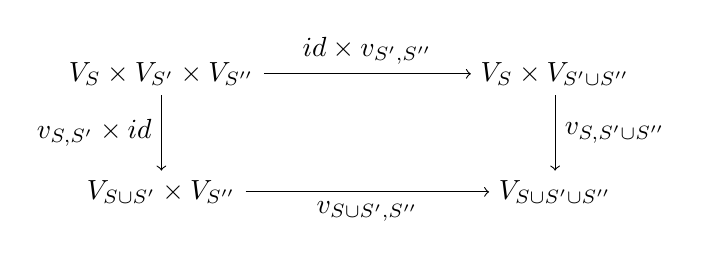
\begin{tikzpicture}
		\node (LT) at (0, 1.5) {$V_S \times V_{S'} \times V_{S''}$};
		\node (LB) at (0, 0) {$V_{S \cup S'} \times V_{S''}$};
		\node (RT) at (5, 1.5) {$V_S \times V_{S' \cup S''}$};
		\node (RB) at (5, 0) {$V_{S \cup S' \cup S''}$};
		\draw [->] (LT) -- node [left] {$v_{S,S'} \times id$} (LB);
		\draw [->] (LT) -- node [above] {$id \times v_{S', S''}$} (RT);
		\draw [->] (RT) -- node [right] {$v_{S, S' \cup S''}$} (RB);
		\draw [->] (LB) -- node [below] {$v_{S \cup S', S''}$} (RB);
		%\node at (0.5, 1) {$\ulcorner$};
		%\node at (1.5, 0.5) {$\lrcorner$};
	\end{tikzpicture}
	\end{center}
	\end{enumerate} 
	\item The morphisms from $\{ V_S, v_{S, S'} \} \to \{ W_S, w_{S, S'} \}$ consist of collections of linear maps $\{ \phi_S: V_S \to W_S \}$, such that $\phi_{\emptyset} = id$ and for each pair of disjoint subsets $S, S' \subseteq B$ the following square commutes:
	\begin{center}
	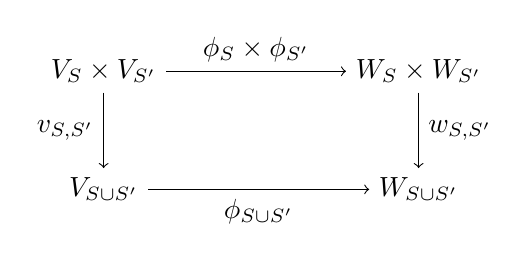
\begin{tikzpicture}
		\node (LT) at (0, 1.5) {$V_S \times V_{S'}$};
		\node (LB) at (0, 0) {$V_{S \cup S'}$};
		\node (RT) at (4, 1.5) {$W_S \times W_{S'}$};
		\node (RB) at (4, 0) {$ W_{S \cup S'}$};
		\draw [->] (LT) -- node [left] {$v_{S,S'}$} (LB);
		\draw [->] (LT) -- node [above] {$\phi_S \times \phi_{S'}$} (RT);
		\draw [->] (RT) -- node [right] {$w_{S,S'}$} (RB);
		\draw [->] (LB) -- node [below] {$\phi_{S \cup S'}$} (RB);
		%\node at (0.5, 1) {$\ulcorner$};
		%\node at (1.5, 0.5) {$\lrcorner$};
	\end{tikzpicture}.
	\end{center}
\end{itemize} \CD{Do we want full stops at the end of display diagrams like this, and if so, at the bottom or centered?}
Thus an object of $\Vect(A)$ consist partly of an $A$-tuple of vector spaces, namely $ (V_{\{a\}})_{a \in A}$. Each vector space $V_S$ should then be thought of as a {\em choice} of simultaneous tensor product of all the $V_{\{a\}}$ where $a \in S$. The data and conditions of an object of $\Vect(A)$ make this intuitive description precise, and similarly for the morphisms of $\Vect(A)$. 

The assignment $A \mapsto \Vect(A)$ gives a functor $\Vect: \Gamma^{op} \to \Cat$, for if $f: A \to P(B)$, then we obtain a functor $f^*: \Vect(B) \to \Vect(A)$ as follows. If $T \subseteq A$, let $f(T) = \cup_{a \in T} f(a) \subseteq B$. Then an object $\{ V_S, v_{S,S'} \}_{S, S' \subseteq B}$ of $\Vect(B)$ is sent via $f^*$ to the object $\{ W_T, w_{T, T'} \}_{T, T' \subseteq A} \in \Vect(A)$, where 
\begin{equation*}
	W_T = V_{f(T)} \quad \textrm{and} \quad  w_{T, T'} = v_{f(T), f(T')}.
\end{equation*}
This assignment is strictly compatible with composition in $\Gamma^\text{op}$. Moreover, since the tensor product is defined by a universal property, the forgetful functor $\Vect(A) \to \Vect^{\times |A|}$ is an equivalence of categories, as desired.  

\section{Composition via the category $\Delta$} \label{sec-Compdelta}


%\NS{As discussed in email, this subsection should have an expository paragraph near the beginning incorporating some of the motivational material currently in the next section}

In the last section we described how symmetric monoidal structures may be encoded through the use of the category $\Gamma$. In this section we will describe a similar process in which the composition in a category may be described through the use of combinatorial simplex category $\Delta$. 
%\CSPcomm{Iterating this idea leads to the notion of {\em Segal $n$-category}, and incorporating our insights about $\Gamma$ yields a notion of symmetric monoidal $(\infty,3)$-category.  }

\begin{definition}
	The simplex category $\Delta$ is a skeleton of the category of finite non-empty totally ordered sets and order preserving maps. The objects of $\Delta$ are the ordered sets $[n] = \{ 0 < 1 < 2 < \cdots < n\}$. 
\end{definition}

The simplex category plays a dual role which sometimes results in confusing terminology. On the one had it has a geometric interpretation as the category of combinatorial simplices. This gives rise to terminology such as a {\em $k$-simplex} of $[n]$, which is a strictly order preserving map $[k] \to [n]$. There are $ {n+1}\choose {k+1}$ such maps. The $0$-simplices will be called {\em vertices} and $1$-simplices will be called {\em edges}. \CD{I think this paragraph can be removed, then add defs of vertices and edges where needed; or did I miss where this confusion comes up for us?}

But there are other aspects of $\Delta$ which come from its description as a category of certain totally ordered sets. The vertices of $[n]$ have a natural ordering induced from the ordering of $[n]$. Let $[m + n]$ denote the ordered concatenation of $[m]$ with $[n]$. We thus obtain the following commuting square, 
\begin{equation} \label{Eqn:Segal-Co-Map}  
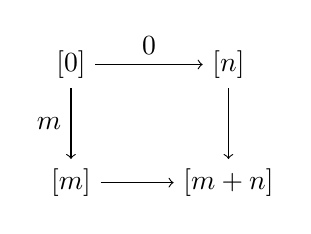
\begin{tikzpicture}[baseline = 0.75cm]
	\node (LT) at (0, 1.5) {$[0]$};
	\node (LB) at (0, 0) {$[m]$};
	\node (RT) at (2, 1.5) {$[n]$};
	\node (RB) at (2, 0) {$[m+n]$};
	\draw [->] (LT) -- node [left] {$m$} (LB);
	\draw [->] (LT) -- node [above] {$0$} (RT);
	\draw [->] (RT) -- node [right] {$$} (RB);
	\draw [->] (LB) -- node [below] {$$} (RB);
	%\node at (0.5, 1) {$\ulcorner$};
	%\node at (1.5, 0.5) {$\lrcorner$};
\end{tikzpicture}
\end{equation}\CD{I think we'll want to label this diagram with a letter, say S, because there are so few number references.}
where $0: [0] \to [n]$ and $m: [0] \to [m]$ denote the first and last vertices, respectively. This square will play an important role in what follows. 

Just as a monoid may be described as a certain presheaf on $\Gamma$, a category may be described as a certain presheaf on $\Delta$, called the {\em nerve} of the category. \CD{I feel like we might as well say explicitly what `presheaf' means, and I'm also slightly concerned that we shift back and forth between `presheaf on $\Delta$' and `simplicial object' at times without any (discernable to me just now) reason.}
This well-known construction proceeds as follows: each ordered set $[n] \in \Delta$ may be viewed as a category (the objects are the elements of $[n]$, with a unique morphism from $i$ to $j$ if $i \leq j$). Thus if $X$ is a category, we obtain a presheaf $NX$ of sets on $\Delta$ by the assignment $[n] \mapsto NC_n = Fun([n], X)$, the set of functors from $[n]$ to $X$.    
The $n^\textrm{th}$ set of $NX_{\bullet}$ is given by the formula
\begin{equation*}
	NX_n := \sqcup_{x_0, x_1, \dots, x_n \in X_0} \Hom_X(x_0, x_1) \times \Hom_X(x_1, x_2) \times \cdots \times \Hom_X(x_{n-1}, x_n).
\end{equation*} 
In other words $NC_n$ consists of all length-$n$ strings of composable morphisms of $X$.

The nerve construction is a fully-faithful functor from categories and functors to the category of presheaves. Moreover the essential image of the nerve construction consists of those presheaves $X$ on $\Delta$  such that the squares induced by those in equation (\ref{Eqn:Segal-Co-Map}),
\begin{center}
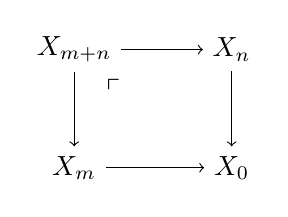
\begin{tikzpicture}
	\node (LT) at (0, 1.5) {$X_{m+n}$};
	\node (LB) at (0, 0) {$X_m$};
	\node (RT) at (2, 1.5) {$X_n$};
	\node (RB) at (2, 0) {$X_0$};
	\draw [->] (LT) -- node [left] {$$} (LB);
	\draw [->] (LT) -- node [above] {$$} (RT);
	\draw [->] (RT) -- node [right] {$$} (RB);
	\draw [->] (LB) -- node [below] {$$} (RB);
	\node at (0.5, 1) {$\ulcorner$};
	%\node at (1.5, 0.5) {$\lrcorner$};
\end{tikzpicture}
\end{center} \CD{Caret in that corner or the other?}
are a pullback diagrams. 

This can be extended to categories internal to a category $C$. \CD{There is something amiss around here --- the above two paragraphs and this paragraph cover similar ground (eg introducing simplicial objects and notation for such), with the latter paragraphs being more elementary.  Was the latter stuff meant to be deleted when the above was added? Or maybe this stuff should move higher up?}
The category of {\em simplicial objects of $C$} is the functor category $Fun(\Delta^\textrm{op}, C) = sC$. We write $X_\bullet$ for such a functor, and let $X_n$ denote the value assigned $[n] \in \Delta$. A {\em category internal to $C$} is a simplicial object $X$, such that the diagrams induced by those in equation (\ref{Eqn:Segal-Co-Map}),
\begin{center}
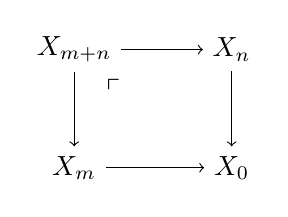
\begin{tikzpicture}
	\node (LT) at (0, 1.5) {$X_{m+n}$};
	\node (LB) at (0, 0) {$X_m$};
	\node (RT) at (2, 1.5) {$X_n$};
	\node (RB) at (2, 0) {$X_0$};
	\draw [->] (LT) -- node [left] {$$} (LB);
	\draw [->] (LT) -- node [above] {$$} (RT);
	\draw [->] (RT) -- node [right] {$$} (RB);
	\draw [->] (LB) -- node [below] {$$} (RB);
	\node at (0.5, 1) {$\ulcorner$};
	%\node at (1.5, 0.5) {$\lrcorner$};
\end{tikzpicture}
\end{center}
are a pullback diagrams. For a general simplicial object $X$, these commuting squares will be called {\em Segal squares} and if they are pullback squares we will say that $X$ satisfies the {\em Segal condition}. Hence a category internal to $C$ is a simplicial object satisfying the Segal condition. \CD{Note to self: at some point, actually set this crucial notion out in a display, perhaps just for $C = Set$.}

This may be contrasted with the notion of a category enriched to $C$, which consists of a {\em set} of objects together with hom objects $\Hom(x,y) \in C$ (as opposed to an object $X_0 \in C$ of ``objects''). Under certain conditions these notions may be related. A category is {\em extensive} (or {\em infinitary extensive}) if it admits small coproducts and coproducts are disjoint and stable under pullback. If $C$ is an extensive category with a terminal object, then a category enriched in $C$ is merely an internal category $X$ in which the object $X_0$ is {\em discrete}, i.e. a coproduct of terminal objects. Examples of extensive categories with terminal objects include the categories of sets, any category of presheaves (or more generally any Grothendieck topos), the category of topological spaces, and the category of small categories. 

\begin{example}
	An ordinary (small) category is a category enriched in sets.
\end{example}

\begin{example}
	A {\em strict 2-category} is a category enriched in categories.
\end{example}

Thus a strict 2-category may equivalently be regarded as a simplicial object with values in $\Cat$, such that $X_0$ is a set (thought of as a discrete category), and such that the Segal squares are pullback squares. Since $X_0$ is a set, these pullbacks may be simultaneously regarded as pullbacks in the 1-category of categories and functors or as weak (or homotopy) pullbacks in the 2-category of categories, functors, and natural transformations. If $X_0$ is allowed to be a general category, these two notions of pullback may differ. 



We would now like to use this insight to describe higher categories. \CD{(specify which insight)} Heuristically an $n$-category is a category enriched in $(n-1)$-categories, and so we should be able to describe it as a discrete presheaf on $\Delta$ with values in the category of $(n-1)$-categories. \CD{Is `discrete presheaf' proper terminology?} The element $[n] \in \Delta$ should be mapped to the $(n-1)$-category of all length-$n$ composable strings of $1$-morphisms. 

However, unless our $n$-category is strict this naive attempt will fail to produce a functor out of $\Delta$. The reasons are analogous to the previous situation with symmetric monoidal structures. However, the insights in the previous section also suggests a possible solution. Rather than require $X_{m+n}$ to be {\em isomorphic} to the pullback $X_m \times_{X_0} X_n$, we require that it merely be {\em equivalent} to the pullback. 
Following this reasoning gives rise to the notion of weak $n$-category first proposed by Tamsamani \cite{Tamsamani:thesis}.   

\begin{definition}[Sketch]
	A Tamsamani $0$-category is a set. 	A {\em Tamsamani $n$-category} is a simplicial object in $(n-1)$-fold simplicial sets, such that the following conditions are satisfied: \CD{Define $(n-1)$-fold simplicial set.}
	\begin{enumerate}
		\item The $(n-1)$-fold simplicial set $X_0$ is constant and discrete.
		\item Each of the $(n-1)$-fold simplicial sets $X_k$ is a Tamsamani $(n-1)$-category.
		\item For every $i$ and $j$, the Segal square,
		\begin{center}
		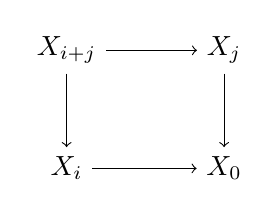
\begin{tikzpicture}
			\node (LT) at (0, 1.5) {$X_{i+j}$};
			\node (LB) at (0, 0) {$X_i$};
			\node (RT) at (2, 1.5) {$X_j$};
			\node (RB) at (2, 0) {$X_0$};
			\draw [->] (LT) -- node [left] {$$} (LB);
			\draw [->] (LT) -- node [above] {$$} (RT);
			\draw [->] (RT) -- node [right] {$$} (RB);
			\draw [->] (LB) -- node [below] {$$} (RB);
			%\node at (0.5, 1) {$\ulcorner$};
			%\node at (1.5, 0.5) {$\lrcorner$};
		\end{tikzpicture}
		\end{center}
		induces an {\em equivalence} $X_{i+j} \to X_i \times_{X_0} X_j$ of Tamsamani $(n-1)$-categories.
	\end{enumerate}
\end{definition} \CD{I think we should spell this definition out for $n=1$, just to make contact with the earlier discussion.}

\noindent To make this precise, one must also inductively build the notation of equivalence. We will do this in the next section, where we describe Segal $n$-categories, the $(\infty,n)$-variant of this construction where instead of working with simplicial sets we use simplicial spaces; Segal $n$-categories were first defined by Hirschowitz and Simpson \cite{9807049}. Tamsamani $n$-categories may then be identified with the {\em discrete} Segal $n$-categories.  It is well-known that the theory of Tamsamani 2-categories forms a good model for the theory of bicategories. This is discussed in detail in \cite{MR2366560}.


\section{Model categories of symmetric monoidal $(\infty,n)$-categories} \label{sec-symmoninftyNcat}

\CDcomm{Proposal: everything from this section except the definition of Segal $n$-category and necessary preliminaries for that is moved into an appendix.  (``Comparison of Segal $n$-categories and $n$-fold complete Segal spaces".)}

\CSP{do we need a review of model categories?}

In this section we will briefly review two theories of $(\infty,n)$-categories which play a role in the current work. These are the Quillen model categories of {\em $n$-fold complete Segal spaces} (due to Barwick) and of {\em Segal $n$-categories}. Both may be constructed inductively, beginning with the standard Kan model structure on simplicial sets. Symmetric monoidal variants of these theories will also be explained. 

In the case $n=1$, the first appearance of Segal categories in the literature is in a paper of Dwyer, Kan, and Smith \cite{MR984042}, where they are called special $\Delta^\op$-diagrams. The concept was adapted and iterated by Tamsamani \cite{Tamsamani:thesis} in order to construct a notion of weak $n$-category. This was then turned into the notion of Segal $n$-categories by Hirschowitz and Simpson \cite{9807049}. The construction is inductive.  First the model structure of Segal $(n-1)$-categories is constructed, then a model structure is constructed on Segal $n$-precategories (described below) in which the fibrant objects are the Segal categories {\em enriched in Segal $(n-1)$-categories}. This raises the question of whether one may form a model category of Segal categories enriched in a general model category? This was addressed in Pelissier's thesis \cite{Pelissier:thesis} with further improvements by Simpson \cite{1001.4071}.  

Complete Segal spaces were introduced by Rezk \cite{MR1804411} as a model for the {\em homotopy theory of homotopy theories}.  A general method of iterating the construction of complete Segal spaces was first given by Barwick \cite{Barwick:thesis}, and recalled, with some additional improvements, by Lurie \cite{0905.0462, MR2555928}. This again can be accomplished quite generally and there are constructions at both the model category and $\infty$-category level. 

The theory of $n$-fold complete Segal spaces figures prominently in the proof of the cobordism hypothesis \cite{MR2555928}, while the theory of Segal $n$-categories provides a more convenient model in which to construct the symmetric monoidal $(\infty,3)$-category of tensor categories, a task we take up in Section \ref{sec-tc-threecat}. We wish to be able to apply the results of \cite{MR2555928} directly to this symmetric monoidal $(\infty,3)$-category and for this we need to understand the relationship between these two model categories. We describe the comparison in this section, and in the following section we describe how to see the invariance of the dualizability filtration.  \CD{If we keep the section on dualizability, this will need explaning.}

\begin{definition}
	Let $\sSet$ denote the category of simplicial sets. An {\em $n$-fold simplicial space} is a functor $X: (\Delta^\textrm{op})^{\times n} \to \sSet$. A {\em $\Gamma$-$n$-fold simplicial space} is a functor $X: \Gamma^\textrm{op} \times (\Delta^\textrm{op})^{\times n} \to \sSet$.
\end{definition}

\begin{definition}
		A $0$-fold simplicial space (i.e. a simplicial set) is a {\em $0$-fold complete Segal space} if it is a Kan complex. An $n$-fold simplicial space $X$, regarded as a simplicial object $X_\bullet$ in $(n-1)$-fold simplicial spaces is an {\em $n$-fold complete Segal space} if it is Reedy fibrant and the following conditions are satisfied:
		\begin{enumerate}
			\item The $(n-1)$-fold simplicial space $X_0$ is {\em essentially constant}, i.e. the induced $(n-1)$-fold simplicial object in the homotopy category of spaces is constant. 
			\item Each of the $(n-1)$-fold simplicial spaces $X_k$ is an $(n-1)$-fold complete Segal space.
			\item For every $m$ and $n$, the Segal square,
			\begin{center}
			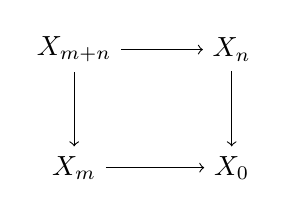
\begin{tikzpicture}
				\node (LT) at (0, 1.5) {$X_{m+n}$};
				\node (LB) at (0, 0) {$X_m$};
				\node (RT) at (2, 1.5) {$X_n$};
				\node (RB) at (2, 0) {$X_0$};
				\draw [->] (LT) -- node [left] {$$} (LB);
				\draw [->] (LT) -- node [above] {$$} (RT);
				\draw [->] (RT) -- node [right] {$$} (RB);
				\draw [->] (LB) -- node [below] {$$} (RB);
				%\node at (0.5, 1) {$\ulcorner$};
				%\node at (1.5, 0.5) {$\lrcorner$};
			\end{tikzpicture}
			\end{center}
			induces a level-wise \CD{Explain exactly what `level-wise' means here.}
			equivalence of $(n-1)$-fold simplicial spaces $X_{m+n} \to X_m \times_{X_0} X_n$.
			\item The simplicial space $X_{k, 0 \dots, 0}$ is a complete Segal space for all $k\geq 0$. 
		\end{enumerate}
\end{definition}

\begin{theorem}[\cite{Barwick:thesis, 0905.0462, 1112.0040}]
	There is a left proper combinatorial simplicial model category structure on $n$-fold simplical spaces in which the fibrant objects are the $n$-fold complete Segal spaces. This model category arrises as a left Bousfield localization of the Reedy (a.k.a. injective) model structure on $n$-fold simplical spaces. \CD{Injective??}
\end{theorem}

\noindent We will denote the model category of $n$-fold complete Segal spaces by $\CSS_n$.  \CD{Presumably the objects are $n$-fold simplicial spaces; need to make it clear that that is the intention, not restricting to the fibrant objects.  Similarly for Segal categories below.}

\begin{definition}
	A $0$-fold simplicial space (i.e. a simplicial set) is a {\em  Segal $0$-category} if it is a Kan complex. An $n$-fold simplicial space $X$, regarded as a simplicial object $X_\bullet$ in $(n-1)$-fold simplicial spaces is an {\em Segal $n$-category} if it is Reedy fibrant and the following conditions are satisfied:
		\begin{enumerate}
			\item The $(n-1)$-fold simplicial space $X_0$ is constant and discrete.
			\item Each of the $(n-1)$-fold simplicial spaces $X_k$ is a  Segal $(n-1)$-category.
			\item For every $m, n$, the Segal square,
			\begin{center}
			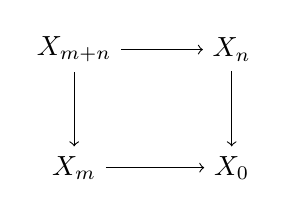
\begin{tikzpicture}
				\node (LT) at (0, 1.5) {$X_{m+n}$};
				\node (LB) at (0, 0) {$X_m$};
				\node (RT) at (2, 1.5) {$X_n$};
				\node (RB) at (2, 0) {$X_0$};
				\draw [->] (LT) -- node [left] {$$} (LB);
				\draw [->] (LT) -- node [above] {$$} (RT);
				\draw [->] (RT) -- node [right] {$$} (RB);
				\draw [->] (LB) -- node [below] {$$} (RB);
				%\node at (0.5, 1) {$\ulcorner$};
				%\node at (1.5, 0.5) {$\lrcorner$};
			\end{tikzpicture}
			\end{center}
			induces an equivalence of  Segal $(n-1)$-categories $X_{m+n} \to X_m \times_{X_0} X_n$.  
				\end{enumerate}
\end{definition}

\noindent This definition is not complete without specifying the notion of equivalence. Fortunately, equivalences between Segal $n$-categories have a relatively direct inductive description as well. This notion of equivalence generalizes to higher dimensions the {\em Dwyer-Kan equivalences}. The $(n-1)$-fold simplicial space $X_0$ is constant and so may be regard as a set, the {\em set of objects} of the Segal $n$-category $X$. 
Inductively one may define three functorial constructions:
\begin{itemize}
	\item For every pair of objects $a,b \in X_0$, an Segal $(n-1)$-category $\Hom_X(a,b)$.
	\item An ordinary category $\mathit{h}X$, called the {\em homotopy category} of $X$.
	\item A set $\pi_0 X$, the set of isomorphism classes of objects of $\mathit{h}X$. 
\end{itemize}
Once we have these constructions, equivalences of Segal $n$-categories are defined as those maps $f:X \to Y$ of $n$-fold simplicial spaces which induce bijections $\pi_0 f: \pi_0 X \to \pi_0 Y$, 
% equivalences of homotopy categories $\mathit{h}f:\mathit{h}X \to \mathit{h}Y$ 
and which induce equivalences of Segal $(n-1)$-categories $\Hom_X(a,b) \to \Hom_Y(fa, fb)$ for every pair of objects $a,b \in X_0$. By construction we see that such maps also induce equivalences $\mathit{h}f:\mathit{h}X \to \mathit{h}Y$.

Given a pair objects $a,b \in X_0$ in an  Segal $n$-category $X$, the  Segal $(n-1)$-category $\Hom_X(a,b)$ is defined to be the fiber \CD{Fiber in what category? Strict or weak? Levelwise?}
over $(a,b) \in X_0 \times X_0$ of the map $(d_0, d_1): X_1 \to X_0 \times X_0$.  
\begin{center}
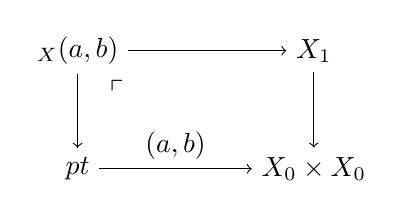
\begin{tikzpicture}
	\node (LT) at (0, 1.5) {$\Hom_X(a,b)$};
	\node (LB) at (0, 0) {$pt$};
	\node (RT) at (3, 1.5) {$X_1$};
	\node (RB) at (3, 0) {$X_0\times X_0$};
	\draw [->] (LT) -- node [left] {$$} (LB);
	\draw [->] (LT) -- node [above] {$$} (RT);
	\draw [->] (RT) -- node [right] {$$} (RB);
	\draw [->] (LB) -- node [above] {$(a,b)$} (RB);
	\node at (0.5, 1) {$\ulcorner$};
	%\node at (1.5, 0.5) {$\lrcorner$};
\end{tikzpicture}
\end{center}
\CD{I think we'll be able to make the induction clearer here, just by indicating exactly what we have and what's being built.  As is there's a danger of it looking circular, just because the induction was split into two pieces.}
The homotopy category $\mathit{h}X$ has the same object set $X_0$, and the morphisms set between two objects is given as the set $\Hom_{\mathit{h}X}(a,b) := \pi_0 \Hom_X(a,b)$. \CD{Need to explain what $\pi_0$ means here.} For every triple of objects $a,b,c \in X_0$ we have a similar  Segal $(n-1)$-category $\Hom_X(a,b,c)$ which is defined as the fiber in $X_2$ over the point $(a,b,c)$ in $X_0 \times X_0 \times X_0$. Since $X$ is an  Segal $n$-category we have induced maps of  Segal $(n-1)$-categories,
\begin{equation*}
	\Hom_X(a,b) \times \Hom_X(b,c) \stackrel{\simeq}{\longleftarrow} \Hom_X(a,b,c) \stackrel{}{\longrightarrow} \Hom_X(a,c).
\end{equation*}
Composition in $\mathit{h}X$ is given by the induced map of sets,
\begin{equation*}
	 \Hom_{\mathit{h}X}(a,b) \times \Hom_{\mathit{h}X}(b,c) \cong \pi_0 \Hom_X(a,b,c)\to \pi_0 \Hom_X(a,c) = \Hom_{\mathit{h}X}(a,c),
\end{equation*}
which is readily seen to be associative. This completes the inductive definition. Just as for $n$-fold complete Segal spaces, there is a model category whose fibrant objects are the Segal $n$-categories. This model structure lives on the category of Segal $n$-precategories, which is defined inductively as follows:

\begin{definition}
	A {\em Segal $0$-precategory} is a simplicial set. {\em Segal $n$-precategory} is an $n$-fold simplicial space $X$, regarded as a simplicial object $X_\bullet$ in $(n-1)$-fold simplicial spaces, such that $X_0$ is constant and discrete and such that each $X_k$ is a  Segal $(n-1)$-precategory. 
\end{definition}

\begin{theorem}[\cite{9807049, Pelissier:thesis, 0905.0462, 1001.4071}] %\CSP{cite \cite{0905.0462}?}
	There is a cartesian left proper combinatorial model structure on the Segal $n$-precategories in which the cofibrations are the monomorphisms, the fibrant objects are the Segal $n$-categories, and the weak equivalences between fibrant objects are the generalized Dwyer-Kan equivalences described above. 
\end{theorem}

\noindent We will denote the above model category of Segal $n$-categories by $\Seg_n$.  \CD{Same issue with underlying objects v. fibrant objects.} Given a Segal $n$-precategory, we may regard it as a $n$-fold simplicial space, and this gives rise to an adjunction \CD{We'll need to explain this adjunction more.}
\begin{equation} \label{Eqn-SegCSS}
	L:\Seg_n \leftrightarrows \CSS_n:R.
\end{equation}
%We would like to thank Clark Barwick for making us aware of the following result and its proof, which shows, in particular, that two Segal $n$-categories give rise to weakly equivalent $n$-fold complete Segal spaces only if they are weakly equivalent as Segal $n$-categories. 
\begin{theorem} \label{thm:SegnCSSnQuillenEquiv}
	The above adjunction is a Quillen equivalence between the model categories of Segal $n$-categories and $n$-fold complete Segal spaces. 
\end{theorem}

\begin{proof}
	In the case $n=1$, this is a result of Bergner \cite[Thm 6.3]{MR2321038} and forms part of one of the first significant comparison results in the subject. In the general case it is clear the functor $L$ preserves monomorphisms, hence cofibrations. To show that $(L,R)$ is a Quillen adjunction, it thus suffices to show that $L$ preserves weak equivalences. This was shown in \cite[Lem. 2.3.13]{0905.0462} for the left adjoint $L: \Seg_{\cA} \to \CSS_{\cB}$ between the $\cA$-enriched Segal category and $\cB$-enriched compete Segal model categories, but only in the special case where $\cA = \cB$ is a sufficiently nice cartesian simplicial combinatorial model category. In fact the identical proof works (by induction) when $\cA = \Seg_{n-1}$ and $\cB= \CSS_{n-1}$.  
	
	Hence to show (\ref{Eqn-SegCSS}) is a Quillen equivalence it is enough to show that this Quillen adjunction induces an equivalence of homotopy categories. 
	If follows from \cite[Thm. 12.6, Ex. 13.8]{1112.0040} that both $\Seg_n$ and $\CSS_n$ are models for the {\em homotopy theory of $(\infty,n)$-categories}. In particular they have equivalent underlying  $(\infty,1)$-categories, and moreover they are generated by the {\em cells} under (homotopy) colimits. The derived functors of the above Quillen adjunction form an adjunction between underlying $(\infty,n)$-categories:
	\begin{equation*}
		\LL L : \Seg_n^{\circ} \leftrightarrows \CSS_n^{\circ}: \RR R.
	\end{equation*} 
The left adjoint $\LL L$ is easily seen to preserve the {cells} (the original left adjoint $L$ has this property and the cells are fibrant-cofibrant objects), and since it also preserves homotopy colimits it follows that $\LL L$ is an equivalence. In particular $L$ induces an equivalence of homotopy categories. 	
\end{proof}

%
%The above result follows by combining several previously known results. The model category of Segal $n$-categories, due originally to Hirschowitz and Simpson \cite{9807049} and based on Tamsamani's notion of weak $n$-category \cite{Tamsamani:thesis}, is constructed iteratively. First the model structure of Segal $(n-1)$-categories is constructed, then a model structure is constructed on Segal $n$-precategories in which the fibrant objects are the Segal categories {\em enriched in Segal $(n-1)$-categories}. This raises the question of whether one may form a model category of Segal categories enriched in a general model category? This was addressed in Pelissier's thesis \cite{Pelissier:thesis} with further improvements by Simpson \cite{1001.4071}, leading the following result:  
%\begin{theorem}[{\cite[Thm. 21.3.2]{1001.4071}}]
%	If $\cM$ is a tractable left proper cartesian model category, then there is a model category structure $\Seg_{\cM}$ on $\cM$-enriched Segal precategories in which the fibrant objects are the (Reedy fibrant) $\cM$-enriched Segal categories. The model category $\Seg_{\cM}$ is again  tractable, left proper, and cartesian. 
%\end{theorem}	
%\noindent Here {\em tractable} is an improvement (due to Clark Barwick) on Jeff Smith's notion of combinatorial model category. In the case at hand we will only need to consider combinatorial $\cM$ in which the cofibrations are the monomorphisms, in which case $\cM$ is automatically tractable. 
%
%
%Complete Segal spaces were introduced by Rezk \cite{??Rezk} as a model for the {\em homotopy theory of homotopy theories}.  A general method of iterating the construction of complete Segal spaces was first given by Barwick \cite{Barwick:thesis}, and recalled, with some additional improvements, by Lurie \cite{0905.0462, MR2555928}. This again can be accomplished quite generally and there are constructions at both the model category and $\infty$-category level.  	
%\begin{theorem}[{\cite[Prop 1.5.4]{0905.0462}}]
%	Let $\cM$ be a left proper simplicial combinatorial model category which is an {absolute distributor}. Then the category $\Fun(\Delta^\op, \cM)$, of simplicial objects in $\cM$, admits the $\cM$-enriched complete Segal model structure $\CSS_{\cM}$. Moreover the model structure $\CSS_{\cM}$ is again left proper, simplicial, combinatorial, and an absolute distributor.
%\end{theorem}	
%\noindent The condition of being an {\em absolute distributor} is needed in order to formulate the correct notion of {\em complete} $\cM$-enriched Segal object. We will not need specifics of this condition and so refer the reader to \cite{0905.0462} for details, but we do note that being an absolute distributor is a property of the $(\infty,1)$-category underlying the given model category. In particular it is preserved under any Quillen equivalence. Moreover this construction is functorial: a Quillen equivalence $\cM \leftrightarrows \cN$ induces a Quillen equivalence $\CSS_{\cM} \leftrightarrows \CSS_{\cN}$.
%
%Thus we have two iterative constructions of theories of $(\infty,n)$-categories, which may both be seeded with the model category of simplicial sets. It is natural to try to compare them. Complete Segal spaces were  shown to be equivalent to Segal categories in work of Bergner \cite{Bergner??}. 
%\CSP{For the equivalence of Segal 1-cats to complete Segal spaces I might also mention Joyal-Teirney and Toen?}
%Lurie \cite{0905.0462} has generalized Bergner's work. He gives criteria on a left proper combinatorial simplicial model category $\cM$ which permit us to construct a model structure on $\cM$-enriched Segal precategories $\Seg_{\cM}$, such that the adjunction 
%\begin{equation*}
%	\Seg_{\cM} \leftrightarrows \CSS_{\cM}
%\end{equation*}
%is a Quillen equivalence. These criteria include, of course, the requirement that $\cM$ is an absolute distributor. We recall a special case:
%\begin{theorem}[{\cite[Prop. 2.3.1, Prop 1.5.10]{0905.0462}}]
%	Let $\cM$ be a left proper combinatorial simplicial model category in which the cofibrations are the monomorphisms, in which weak equivalences are stable under filtered colimits, and which is Quillen equivalent to $\CSS_{n-1}$. Then there exists a left proper combinatorial  model category structure on $\cM$-enriched Segal precategories $\Seg_{\cM}$ such that the fibrant objects are the injective fibrant $\cM$-enriched Segal categories, such that the weak equivalences are stable under filtered colimits, and such that the canonical adjunction
%	\begin{equation*}
%		\Seg_{\cM} \leftrightarrows \CSS_{\cM}
%	\end{equation*} 
%	is a Quillen equivalence.
%\end{theorem} 
%\noindent In particular $\Seg_{\cM}$ will be Quillen equivalent to $n$-fold complete Segal spaces $\CSS_n$. 
%
%\begin{proof}[Proof of Theorem \ref{thm:SegnCSSnQuillenEquiv}]
%	The above results go most of the way to showing that Segal $n$-categories are Quillen equivalent to $n$-fold complete Segal spaces. However there are still a few minors points to discuss. The assumptions Simpson and Lurie place on the model category $\cM$ used to construct $\Seg_{\cM}$ are slightly different, though when both sets of conditions are satisfied they give rise to the same model categories. The most important difference is that Simpson assumes that $\cM$ is a {\em cartesian} model category, while Lurie assumes that $\cM$ is {\em simplcial}. In general $\Seg_{\cM}$ will not be a simplicial model category even if $\cM$ is simplicial, and consequently there are difficulties in directly iterating Lurie's construction or applying his results to Simpson's Segal $n$-categories.   
%
%Fortunately there is a way around this. Dugger \cite{??Dugger} has shown that every combinatorial model category $\cM$ is Quillen equivalent to a left proper simplicial combinatorial model category  $\cM'$ in which all objects are cofibrant. Toen  \cite[Prop 2.3(2)]{Toen??} has improved on this, showing that, in particular, when $\cM$ is cartesian,  $\cM'$ will again be cartesian and moreover that the Quillen equivalence is {\em weakly cartesian}. This means that the canonical map $F(X \times Y) \to  F(X) \times F(Y)$ is a weak equivalence for all object $X$ and $Y$. It is clear from Simpon's construction that a weakly cartesian Quillen equivalence $\cM \sim \cN$ induces a Quillen equivalence $\Seg_{\cM} \sim \Seg_{\cN}$. 
%
%Let $\cM$ be the cartesian simplicial replacement for Segal $n$-categories $\Seg_n$. Combining these results (and using induction) gives a chain of Quillen equivalences:
%\begin{equation*}
%	\Seg_{n+1} \sim \Seg_{\cM} \sim \CSS_{\cM} \sim \CSS_{n+1}.
%\end{equation*}
%To see that the specific Quillen adjunction (\ref{Eqn-SegCSS}) is a Quillen equivalence, we need only see that it induces an equivalence on underlying $(\infty,1)$-categories. This follows from the \cite[Thm 12.6]{1112.0040} and the fact that the Quillen adjunction in question preserves the {\em cells}. Alternatively, one may deduce this from a more careful consideration of the steps involved in constructing the cartesian simplicial replacement guaranteed by Dugger and Toen's results. 
%\end{proof}


In particular two Segal $n$-categories give rise to weakly equivalent $n$-fold complete Segal spaces only if they are weakly equivalent as Segal $n$-categories. \CD{only if?}

Both of the model categories $\CSS_n$ and $\Seg_n$ are cofibrantly generated, which \CD{Need transition sentence indicating moving on to symmetric monoidal.}
implies that the functor categories $\Fun(\Gamma^\op, \CSS_n)$ and $\Fun(\Gamma^\op, \Seg_n)$ carry (Quillen equivalent) projective model structures. We may now obtain symmetric monoidal variants of $\CSS_n$ and $\Seg_n$ by taking the left Bousfield localization with respect to the maps \CD{Words of explanation regarding left Bousfield localization?}
\begin{equation*}
	\left(\coprod_{a \in A} i_a\right) :   \coprod_{a \in A} y(1) \to y(A)
\end{equation*}
\CD{Need to reintroduce $A$.}
where $y: \Gamma \to \Fun(\Gamma^\op, \Set) \to \Fun(\Gamma^\op, \Seg_n)$ denotes the Yoneda embedding. These maps co-represent the Segal maps of Section \ref{sec-symmonGamma}. Let $\CSS_n^{\otimes}$ and $\Seg_n^{\otimes}$ denote the corresponding model categories. 
\CSP{Are there better notations?}
The fibrant objects are described in the following definition:


\begin{definition}
	A {\em symmetric monoidal $n$-fold complete Segal space} (respectively {\em symmetric monoidal Segal $n$-category}) is a $\Gamma$-$n$-fold simplicial space $X$, which we view as a functor from $\Gamma^\textrm{op}$ to $n$-fold simplicial spaces, such that the following conditions are satisfied. 
	\begin{enumerate}
		\item $X_A$ is an $n$-fold complete Segal space (resp. Segal $n$-category) for each $A \in \Gamma$. 
		\item For each set $A \in \Gamma$ (possibly empty) the canonical map,
		\begin{equation*}
			\prod_{a \in A} i_a^*: X_A \to \prod_{a \in A} X_{(1)}
		\end{equation*}
		is an equivalence of $n$-fold complete Segal spaces (resp. Segal $n$-categories). 
		%\CSP{Should we also add the $X_{(0)} = pt$? We get $X_{(0)} \simeq pt$ for free.}
	%	\item (optional) The previous axiom implies that $X_\emptyset \simeq pt$. We assert that $X_\emptyset = pt$. 
	\end{enumerate}
\end{definition}


\noindent We now describe a few examples of Segal $n$-categories for small $n$. Recall any map between discrete simplicial sets is a fibration. Hence any discrete $n$-fold simplicial space is Reedy fibrant.




\begin{example}
	A set may be regarded as a constant simplicial space. Thus the nerve of an ordinary category may be regarded as a discrete simplcial space. A discrete simplicial space is a Segal 1-category if and only if it is the nerve $NC$ of an ordinary category $C$. In this case $NC_0 = \textrm{ob}\ C$, the spaces $\Hom_{NC}(a,b)$ are the sets $\Hom_C(a,b)$, and the homotopy category $\mathit{h}NC$ is isomorphic to the original category $C$. If $C$ is symmetric monoidal then, following the discussion in Section \ref{sec-symmonGamma}, the above construction produces a symmetric monoidal Segal 1-category.  \CD{Need to specify ``the above construction".}
\end{example}

\begin{example}
	A strict 2-category $C$ may be regarded as a simplical object $C_\bullet$ in $\Cat$ specified as follows:
	\begin{equation*}
		C_n := \sqcup_{x_0, x_1, \dots, x_n \in C_0} \Hom_C(x_0, x_1) \times \Hom_C(x_1, x_2) \times \cdots \times \Hom_C(x_{n-1}, x_n).
	\end{equation*}
	We obtain a 2-fold simplicial set by applying the nerve construction to each of these categories; by viewing a set as a discrete simplicial space, we regard the result as a 2-fold simplicial space $NC_{\bullet \bullet}$. Since $C_\bullet$ satisfies the Segal condition, one deduces that $NC_{\bullet \bullet}$ is a 2-fold Segal category. \CD{At some point we can shrink all the bullets.}
	%\footnote{Alternatively, one may start with the simplicial category $C_\bullet$, as before and apply the {\em complete Segal space nerve} to each of the categories $C_n$. The $k^\text{th}$ space of this simplicial space $N^{CSS}_\bullet C_n$ is obtained by first constructing the functor category $Fun([k], C_n)$, then throwing away the non-invertible natural transformations, and finally applying the classifying space functor to the resulting groupoid. This alternative has the advantage that it produces a {\em complete} Segal space $N^{CSS} C_n$. However for our purposes these are equivalent constructions as the canonical map $N C_n \to N^{CSS} C_n$ is a weak equivalence in the complete Segal space model structure. 
	%[Cite the Joyal Teinery paper for the Quillen equivalence between Segal spaces and Quasi-categories] } 
Following \cite{MR2366560}, we call the association $C \mapsto NC_{\bullet \bullet}$ the {\em 2-nerve}\footnote{The construction in \cite{MR2366560} applies more generally to arbitrary bicategories, and consequently differs slightly from the one we have described.}.  
\end{example}

\begin{lemma}[\cite{MR2366560}] \label{lma:2catnervereflectsequiv}
	A strict functor of strict 2-categories $F: C \to D$ is a weak equivalence if and only if the induced map of 2-fold Segal categories $NC_{\bullet \bullet} \to ND_{\bullet \bullet}$ is an equivalence. \CD{Either remove ``weak" or need to specify meaning of weak equivalence.}
\end{lemma}
\CD{Why do we need this Lemma?}

%\begin{proof}
%	The functor $F$ is a weak equivalence if and only if 
%	\begin{enumerate}
%		\item it is essentially surjective on object, and
%		\item for every pair of objects $a,b \in C$,  it induces an equivalence of categories $C(a,b) \to D(Fa, Fb)$.
%	\end{enumerate}
%On the other hand, a map of 2-fold Segal spaces $X \to Y$ is an equivalence if and only if
%\begin{enumerate}
%	\item it induces a bijection $\pi_0X \to \pi_0Y$, and
%	\item for every pair of objects $a,b \in X_0$, it induces equivalences of 1-fold Segal spaces $\Hom_X(a,b) \to \Hom_Y(Fa, Fb)$.
%\end{enumerate}
%When $X = NC_{\bullet \bullet}$  is a 2-nerve, $\Hom_X(a,b) \cong NC(a,b)_{\bullet}$, so the second conditions are equivalent. Moreover, $\pi_0 NC_{\bullet \bullet}$ is easily seen to be the collection of equivalence classes of objects of $C$. Thus a functor inducing an equivalence of 2-nerves induces a bijection on equivalence classes of objects. In particular if $F$ induces an equivalence of 2-nerves, it is essentially surjective, and hence a weak equivalence of categories. It remains to see that a weak equivalence of categories necessarily induces a bijection on sets of equivalence classes of object. This follows as a well-known exercise.
%\end{proof}


%%%%% Homotopy Hypothesis Stuff %%%%%
%
%One version of the homotopy hypothesis states that the homotopy theory of spaces resides as a special case of the theory of $(\infty,n)$-categories, namely as the $(\infty,n)$-groupoids. This is known to hold for the models of $(\infty,n)$-category described above. This is trivially satisfied when $n=0$, as the theories of $0$-fold complete Segal spaces and Segal $0$-categories are both identical to the standard model category of simplical sets. More generally, to make this precise we must identify the $(\infty,n)$-groupoids, i.e. the {\em spaces}.
%
%\begin{definition}
%	We inductively define {\em spaces} as follows. Segal $0$-categories and $0$-fold complete Segal spaces are spaces. If $X$ is a Segal $n$-category (respectively an $n$-fold complete Segal space), which we view as a simplial object in $(n-1)$-fold simplicial spaces, then $X$ is a {\em space} if
%	\begin{enumerate}
%		\item The homotopy category $\mathit{h}X$ is a groupoid, and
%		\item Each $\Hom_X(a,b)$ (resp. each $X_k$) is a space. 
%	\end{enumerate}
%	When $X$ is an  $n$-fold complete Segal space we may interpret $\mathit{h}X$ by passing to the associated Segal $n$-category via the Quillen equivalence of Equation \ref{Eqn-SegCSS}.
%\end{definition}
%
%
%\begin{example}
%	An $n$-fold complete Segal space is a space if and only if it is an essentially constant $n$-fold simplcial space. The case $n=1$ follows from \cite{MR1804411}. The general case follows by induction from properties (1)-(4) in the definition of $n$-fold complete Segal space.
%\end{example}
%
%Thus the homotopy hypothesis holds for $n$-fold complete Segal spaces as well as for  Segal $n$-categories. This latter equivalence was already established between discrete Segal $n$-categories and homotopy $n$-types by Tamsamani \cite{Tamsamani:thesis}.


%
%\section{Dualizability in Symmetric Monoidal $(\infty,n)$-Categories} \label{sec-duals}
%
%In this section we will describe how to access the space of fully-dualizble objects in a symmetric monoidal $(\infty,n)$-category, and describe an associated dualizability filtration. We will focus on the case of Segal $n$-categories for which the theory is particularly easy to analyze. We begin with a brief account of dualizability in bicategories and monoidal categories. 
%
%\begin{definition}
%	A 1-morphism $f: a \to b$ in a bicategory $\cC$ is a {\em right dualizable} if it admits a right adjoint, that is there exists a 1-morphism $g: b \to a$ (the {\em right adjoint}) and two 2-morphisms $\eta: id_a \to gf$, $\varepsilon: fg \to id_b$, such that the following identities hold: 
%\begin{align*}
%			(id_{g} \circledcirc \varepsilon  ) \circ (  \eta \circledcirc id_{g}) &= id_{g} \\
%			(\varepsilon \circledcirc id_{f}) \circ (id_{f} \circledcirc \eta) &= id_{f}.
%		\end{align*}
%	Here $\circledcirc$ denotes the horizontal composite of 2-morphisms. Conversely $g$ is left dualizable if it  admits a left adjoint. A bicategory $\cC$ will be called {\em dualizable} if all 1-morphisms are both left and right dualizable.  
%\end{definition} 
%
%A monoidal category may be regarded as a single object bicategory, and so the above definition also provides the notion of dualizable monoidal category.  A dualizable monoidal category is more commonly called {\em rigid}. In a symmetric monoidal category there is no distinction between left and right dualizablility. 
%
%\begin{example} \label{example-grpdisdualizable}
%	Any 2-groupoid, that is bicategory in which all 2-morphisms are invertible and 1-morphisms are weakly invertible, is dualizable. 
%\end{example}
%
%\begin{lemma}
%	For every bicategory $\cC$, there exists a sub-bicategory $\cC^{(d)}$ with the following two properties:
%	\begin{enumerate}
%		\item The inclusion $\cC^{(d)} \subseteq \cC$ is fully-faithful on 2-morphisms, $\cC^{(d)}$ contains every object of $\cC$, and the 1-morphisms of $\cC^{(d)}$ are closed under 2-isomorphism in $\cC$. 
%		\item $\cC^{(d)}$ is dualizable and universal in the sense that for every functor $\cD \to \cC$ with $\cD$ a dualizable bicategory,  there exists a unique factorization $\cD \to \cC^{(d)} \hookrightarrow \cC$.
%	\end{enumerate}
%\end{lemma}
%
%\begin{proof}
%	Consider the poset $\cP$ consisting of all dualizable sub-bicategories of $\cC$ satisfying the closure properties of (1), ordered by inclusion. By Example \ref{example-grpdisdualizable},  $\cP$ is non-empty. Moreover the composite of (left) dualizable 1-morphisms is again (left) dualable, thus the sub-bicategory generated (i.e. closed under (1)) by any two elements of $\cP$ is again an element of $\cP$. It follows that the union over all elements of $\cP$, which we call $\cC^{(d)}$, is daulizable and is the maximal element of $\cP$. The final property follows by noting that any functor $\cD \to \cC$ factors (uniquely) through some dualizable sub-bicategory, hence through an element of $\cP$.
%\end{proof}
%
%
%Given a symmetric monoidal Segal $n$-category $X$, which we regard as an object of the functor category $\Fun(\Gamma^\op, \Seg_n)$,  we may apply the homotopy category functor $\mathit{h}$ level-wise to obtain a strict functor from $\Gamma^\op$ to categories, satisfying the Segal condition. We have seen in Section \ref{sec-symmonGamma} how this may be regarded as symmetric monoidal category structure on $\mathit{h}X$.  
%
%For $n\geq 2$, we may extract a discrete Segal 2-category from a given Segal $n$-category $X$, which we may in turn regard as a bicategory $\mathit{h}_2X$, the {\em homotopy bicategory of $X$}. This may be obtained as follows. First, we regard $X$ as a simplicial object in Segal $(n-1)$-categories. Then we may apply the homotopy category functor levelwise to obtain a simplicial object in the category of categories. Finally applying the nerve yields a discrete 2-fold simplicial space, which is easily seen to be a Segal 2-category. This construction is clearly funcotrial and sends weak equivalences of Segal $n$-categories to equivalences of bicategories.
%
%Choosing a pair of two objects $a,b \in X_0$, we may extract the Segal $(n-1)$-category $\Hom_X(a,b)$. Repeating this construction and the pervious one we obtain an assortment of bicategories associated to any Segal $n$-category. 
%
%\begin{definition}
%	A Segal $n$-category $X$ is {\em $k$-dualizable} ($k\geq 2$) if 
%	\begin{enumerate}
%		\item each $Hom_X(a,b)$ is $(k-1)$-dualizable for each pair of objects $a,b \in X_0$ (this condition is vacuous if $k=2$), 
%		\item $\mathit{h}_2 X$ is a dualizable bicategory. 
%	\end{enumerate}
%Moreover if $X$ is symmetric monoidal, we further require that the symmetric monodial category $\mathit{h} X$ is dualizable. We say that a symmetric monoidal Segal $n$-category $X$ is {\em fully-daulizable} if it is $n$-dualizable.
%\end{definition}
%
%Let $X$ be a Segal $n$-category, which we regard as a simplicial object in Segal $(n-1)$-categories. Let $S \subseteq X_0$ be a subset of the objects of $X$, and let $X'$ denote the simplicial object such that
%	\begin{equation*}
%		X'_k =  X_k \times_{(X_0)^{\times k}} (S)^{\times k}.
%	\end{equation*}
%Then a direct calculation shows that $X'$ is again a Segal $n$-category; the full sub-Segal $n$-category spanned by the collection $S$. 
%
%This construction generalizes. If $X$ is symmetric monoidal and $S$ is a sub-symmetric monoidal category of $\mathit{h}X$, then we may form the full sub-symmetric monoidal Segal $n$-category spanned by the collection $S$. Similarly if $X$ is a Segal $n$-category (with $n\geq 2$) and we have a collection of 1-morphisms of $\mathit{h}_2 X$ that is (weakly) closed under composition,  we may form the sub-Segal $n$-category spanned by this collection.  We will only need these two general cases when (1) the symmetric monoidal subcategory of $\mathit{h}X$ is closed under isomorphism of object or (2) the collection of 2-morphisms of $\mathit{h}_2 X$ is closed under 2-isomorphism. In these special cases the desired result is clear. 
%
%
%Given $k \geq 1$ and a Segal $n$-category $X$, we will obtain a decreasing filtration
%\begin{equation*}
%	X = F^0_k X  \supseteq  F^{1}_kX \supseteq  \cdots \supseteq  F^{k-1}_k X. 
%\end{equation*}
%Where $F^i_kX$ consists of the full sub-symmetric monoidal Segal $n$-category of $F^{i-1}_kX$ whose $(k-i)$-morphisms are dualizable. More precisely this may be defined inductively as follows. We assume that we have defined $F^iY$ for all $0 \leq i \leq k-1$ and all Segal $(n-1)$-categories $Y$, and that this construction is product preserving. Let $X$ be a Segal $(n-1)$-category, which we view as a simplicial object of $\Seg_{n-1}$. For $i < k-1$, we let $F^i_kX$ be defined by applying the previously constructed $F^i_{k-1}$ levelwise (this exist by induction). For $i=k-1$, we define $F^{k-1}_kX$ to be the full sub-Segal $n$-category of $F^{k-2}_kX$ spanned by those 1-morphisms which are dualizable, i.e. spanned by $(\mathit{h}_2 X)^{(d)} \subseteq \mathit{h}_2 X$. The Segal $n$-category $F^{k-1}_kX$ so obtained is $k$-dualizable. 
%
%For symmetric monoidal Segal $n$-categories $X$, this filtration obtain one more layer $F^k_k X \subseteq F^{k-1}_k X$, which is defined by taking the full sub-symmetric monoidal Segal $n$-category spanned by the maximal dualizable sub-symmetric monodial category $(\mathit{h}X)^{(d)} \subseteq \mathit{h}X$. The symmetric monoidal Segal $n$-category $F^k_k X$ is $k$-dualizable in the symmetric monoidal sense and moreover is universal in the sense that any map $Y \to X$ of symmetric monodial Segal $n$-categoeries with $Y$ $k$-dualizable factors through $F_k^k X$. We have $F_n^n X$ is fully-dualizable. 
%
%
%
%
%%A $0$-morphism of a Segal $n$-category is an object of $X$. For $k \geq 1$, a $k$-morphism of a Segal $n$-category $X$ is a $(k-1)$-morphism of one of the hom Segal $(n-1)$-categories $\Hom_X(a,b)$ for some pair of object $a,b \in X_0$. If $k = 1$, we say two 1-morphisms of $X$ are {\em parallel} if they reside in the same hom Segal $(n-1)$-category $\Hom_X(a,b)$. If $k>1$, then two $k$-morphisms are parallel if they are parallel $(k-1)$-morphisms in the same hom Segal $(n-1)$-category $\Hom_X(a,b)$.
%
%%\CSPcomm{To DO
%%\begin{itemize}
%%	\item invariance of the filtration (even under completion). 
%%\end{itemize}}
%
%




\section{Linear categories, tensor categories, and bimodule categories} \label{sec-tc-lincat}

	Let $k$ be a fixed ground field, and let $\Vect_k$ be the category of finite dimensional $k$-vector spaces.   A {\em linear category} is an abelian category with a compatible enrichment over ${\Vect}_k$.  A {\em linear functor} is a right exact additive functor, which is also a functor of $\overline{\Vect}_k$-enriched categories. \CD{Why $\overline{\Vect}$ here?}
	
If $\{\cA_\alpha\}$ denotes a collection of linear categories then a {\em multilinear functor} from $\{\cA_\alpha\}$ into a linear category $\cB$ consists of a functor
\begin{equation*}
	F: \prod \cA_\alpha \to \cB
\end{equation*}
such that $F$ is linear in each variable separately. A linear category will be said to {\em have enough projectives} if every simple object has a projective cover. \CD{Explain 'simple object'; explain 'proj cover'.} 

\begin{warning}
	Unless otherwise stated {\em all linear functors considered in this paper are right exact functors}.  We are aware that this deviates from convention, and offer the following justification. Many of the construction that will be described in this paper, such as the Deligne tensor product of linear categories and the composition of bimodule categories, are only functorial with respect to right exact functors. To avoid littering this paper with the adjective `right exact' it is simpler to define right exactness into the category from the start.  
\end{warning} \CD{Probably will need to change the phrasing of this warning.}

\begin{definition}
	A {\em tensor category} is a linear monoidal category $(\cC, \otimes, 1, \alpha, \lambda, \rho)$ such that the functor $\otimes$ is multilinear. A {\em tensor functor} is a monoidal functor which is also linear.
\end{definition}

\begin{example}
	The category of finite dimensional vector spaces is an example of a tensor category. If $A$ is an algebra object in $\Vect_k$, then the categories of finitely presented left and right modules, $\Mod{A}{}$ and $\Mod{}{A}$, are linear categories. More generally, if $\cC$ is a tensor category and $A$ is an algebra object in $\cC$ (also known as a monoid object), then the categories $\Mod{A}{}(\cC)$ and $\Mod{}{A}(\cC)$ of left and right $A$-module objects in $\cC$ are also linear categories.
\end{example}

\begin{example}
	If $\cM$ is a linear category, then the category of (right exact) linear endofunctors $\Fun(\cM, \cM)$ is a tensor category. 
\end{example}

\begin{definition}
	Let $\cC$ and $\cD$ be tensor categories. A {\em $\cC$-$\cD$-bimodule category} is a bicategory with exactly two objects $x$ and $y$ such that \CD{What kind of bicategory? We probably need to be explicit about what our definition of bicategories, functors, transformations, modifications is?}
	\begin{itemize}
		\item all hom categories are linear categories, 
		\item horizontal composition is multilinear,
		\item the category $\Hom(y,x)$ is empty, and
		\item there are identifications of monoidal categories $\Hom(x,x) \simeq \cD$ and $\Hom(y,y) \simeq \cC$.
	\end{itemize} \CD{hom or Hom?}
	We will often abuse notation and refer to the value $\cM = \Hom(x,y)$ as the bimodule category. If $\cD \simeq \Vect_k$, then $\cM$ is a {\em left module category}. If $\cC \simeq \Vect_k$, then $\cM$ is a {\em right module category}.
\end{definition}
	
Unpacking this definition we see that a left $\cC$-module category is a linear category $\cM$ together with a multilinear functor $\otimes^{\cM}: \cC \times \cM \to \cM$ and natural isomorphisms
%	\CSP{This looks a little gross. I should change it.}
	\begin{align*}
		\alpha: & \;    \otimes^{\cM} \circ \, (\otimes \times id_{\cM}) \cong  \otimes^{\cM} \circ (id_{\cC} \times \otimes^{\cM}) \\
		\lambda: & \; \otimes^{\cM} \circ \, (1 \times id_{\cM}) \cong id_{\cM},
	\end{align*}
%	\begin{align*}
%		\alpha: & \;    [(-) \otimes (-)] \otimes^{\cM} (-)  \cong  (- ) \otimes^{\cM} [ (-) \otimes^{\cM} (-)] \\
%		\lambda: & \; 1 \otimes^{\cM}(-) \cong id_{\cM},
%	\end{align*}	
	satisfying the evident pentagon and triangle identities. 

\begin{definition}		
A {\em $\cC$-$\cD$ bimodule functor} $F:\cM \to \cN$ is a (strong) functor of bicategories such that \CD{'strong' needs to be explained somewhere}
%	\begin{itemize}
		 $F$ is the identity on objects,
		  the restriction of $F$ to each hom category is linear,
		 and $F$ is the identity on $\Hom(x,x)$ and $\Hom(y,y)$.
%	\end{itemize}
A {\em lax} (resp. {\em oplax}) bimodule functor is a lax (resp. oplax) functor of bicategories satisfying the above conditions. All bimodule functors will be assumed strong unless otherwise stated. 
	A {\em bimodule transformation} is a transformation of functors of bicategories, which restricts to the identity on $\Hom(x,x)$ and $\Hom(y,y)$, and such that the component 1-cells are trivial.  \CD{'component 1-cells' needs to be explained somewhere}
\end{definition}
	
%
Bimodule categories, functors, and transformations form a strict 2-category.
%If $\cM$ and $\cN$ are both $\cC$-$\cD$ bimodule categories, then a bimodule functor which restricts to the identity functor on $\cC$ and $\cD$ will be called a {\em $\cC$-$\cD$-bimodule functor}.

\begin{example}
	Every linear category is a $\Vect_k$-$\Vect_k$-bimodule category in an essentially unique way. \CD{Need to say what is meant by 'essentially'}
\end{example}

\begin{example}
	For any algebra object $A$ in a tensor category $\cC$ the categories $\Mod{}{A}(\cC)$ and $\Mod{A}{}(\cC)$ are respectively left and right $\cC$-module categories. 
\end{example}

\begin{example}
	Let $\cM$ and $\cN$ be left $\cC$-module categories. The categories $\Fun_{\cC}(\cM, \cM)$ and $\Fun_{\cC}(\cN, \cN)$ of (right exact) $\cC$-module endofunctors are both tensor categories. The linear category $\Fun_{\cC}(\cM, \cN)$ is a $\Fun_{\cC}(\cN, \cN)$-$\Fun_{\cC}(\cM, \cM)$-bimodule category.   \CD{Would this be true without right exactness?  If so, worth mentioning.}
	%\CSP{Do I have the right convention for the actions here?} \NS{I think you got it backwards.  $\Fun(\cM,\cM)$ left acts on $\cM$ and so its action by precomposition should be a right action} 
\end{example}

\begin{remark}
 	Every left $\cC$-module category is naturally a right $\cC^{mp}$-module category. \CD{Need to explain $mp$ notation.}
\end{remark}

We will also need a slightly more general notion of bimodule morphism to make sense of multilinear bimodule maps. These in turn are used to define the external Deligne tensor product of bimodule categories. 

\begin{definition}
	A {\em twisted bimodule functor} from a $\cC$-$\cD$-bimodule category $\cM$  to $\cC'$-$\cD'$-bimodule category $\cM'$ is a functor of bicatgories from $\cM$ to $\cM'$ which restricts to the identity on objects and is linear on hom categories. A {\em twisted bimodule transformation} between twisted bimodule functors is a transformation of functors of bicategories such that the component 1-cells are trivial.
\end{definition}

Thus a twisted bimodule functor from a $\cC$-$\cD$-bimodule category $\cM$ to a $\cC'$-$\cD'$-bimodule category $\cM'$ consists in part of tensor functors $f:\cC \to \cC'$ and $g:\cD \to \cD'$, and a map of linear categories $\cM \to \cM'$, compatible with the induced module structures. We will say the the twisted bimodule functor {\em extends the tensor functors $f$ and $g$}. 

If we are given a $\cC'$-$\cD'$-bimodule category $\cM'$ and tensor functors $f:\cC \to \cC'$ and $g:\cD \to \cD'$, then we may also form the {\em twisted bimodule category} ${}_f{\cM'}_g$.  The underlying linear category of ${}_f{\cM'}_g$ is $\cM'$, but the actions are by $\cC$ and $\cD$ via the tensor functors $f$ and $g$. A twisted bimodule functor $\cM \to \cM'$ extending $f$ and $g$ is the same as a $\cC$-$\cD$-bimodule functor $\cM \to {}_f{\cM'}_g$.  Later on we will sometimes use the notation ${}_{\langle f \rangle} \cM'_{\langle g \rangle}$ instead of ${}_f{\cM'}_g$, in cases where the functors $f$ and $g$ are themselves unwieldy composites.

With twisted bimodule functors as morphisms, there exists a terminal bimodule category $\cT$. As a bicategory, each of its non-empty hom categories is the terminal linear category. \CD{If said this way, need to specify what the terminal linear category is.} The product of bimodule categories $\cM \times_{\cT} \cM'$ is defined as the fiber product of bicategories over $\cT$.  \CD{I'm confused by either the mathematics or the exposition here; can discuss.}  \CD{Must explain or provide precise reference for fiber product of bicategories.} We will abuse notation and write this as $\cM \times \cM'$. This is again a bicategory with precisely two objects $x$ and $y$. Moreover
\begin{equation*}
	\Hom_{\cM \times \cM'}(a,b) = \Hom_\cM(a,b) \times \Hom_{\cM'}(a,b)
\end{equation*}
for all pairs $a,b \in \{ x,y \}$.

If $\{ \cM_\alpha \}$ is a collection of bimodule categories then a {\em twisted multilinear bimodule functor} from $\{ \cM_\alpha \}$ into a bimodule category $\cN$ is a functor of bicategories
\begin{equation*}
	\prod_{\alpha} \cM_\alpha \to \cN
\end{equation*}
which is the identity on objects, and which is a twisted bimodule functor in each variable. 

\section{Finite linear categories and the Deligne tensor product} \label{sec-tc-deligne}

The goal of this section is to construct the Deligne tensor product, which takes module categories $\cM_\cC$ and ${}_\cC \cN$ and returns a linear category $\cM \boxtimes_\cC \cN$. For simplicity, we will only define this tensor product for categories satisfying certain smallness properties, so we first introduce the notion of finite tensor categories and discuss their properties, following \cite{MR2119143, EGNO}.

\begin{definition} % This is from EGNO Definition 1.18.2.
	A linear category $\cC$ is {\em finite} if 
	\begin{enumerate}
	%	\item $\cC$ has finite dimensional spaces of morphisms;
	% This is redundant since we are enriched over finite vector spaces.
		\item every object of $\cC$ has finite length; \CD{Explain 'finite length'}
		\item $\cC$ has enough projectives, that is every simple object of $\cC$ has a projective cover; and
		\item there are finitely many isomorphism classes of simple objects.  
	\end{enumerate}
\end{definition}

\begin{remark}
A linear category is finite if and only if it is equivalent to the category $\Mod{A}{}$ of finite dimensional modules over a finite dimensional $k$-algebra $A$. \CD{Reference for this remark.}
\end{remark}

The key property of finite tensor categories is that they satisfy the following analog of the adjoint functor theorem.  Although this result is well known, we were unable to find a proof in the literature, so we include one here.

\begin{proposition} \label{prop:AFT}
	Let $\cC$ and $\cD$ be finite linear categories and let $\cG: \cC \rightarrow \cD$  be an additive $\Vect$-enriched functor (not necessarily right exact). Then the following conditions are equivalent: \CD{Earlier, indicate $\Vect = \Vect_k$.}
	\begin{enumerate}
		\item $\cG$ is left exact;  
		\item $\cG$ is left exact and satisfies the following {\em Solution Set Condition:} \\  For each $d \in \cD$ there is a finite set $I$ and a collection of arrows $f_i:d \to \cG(c_i)$ such that every arrow $h:d \to \cG(c)$ can be written as a composite $h = \cG(t) \circ f_i$ for some index $i \in I$ and some $t: c_i \to c$; 
		\item $\cG$ admits an (additive, ${\Vect}$-enriched, right exact) left adjoint.
	\end{enumerate}
\end{proposition}
\begin{proof} This is a variation of the proof given in \cite[V.6.Thm 2]{MR0354798}.
Suppose that $\cG$ admits a left adjoint, $\cF$. Then $\cG$ is itself a right adjoint and hence commutes with all limits. In particular $\cG$ is a left exact functor. Moreover, as $\cF$ commutes with coproducts, it is automatically additive, and as the unit and counit maps of the adjunction of $\cF$ and $\cG$ are linear maps of vector spaces, $\cF$ is also ${\Vect}$-enriched.  \CD{Explain last step of this first paragraph.}


To construct a left adjoint for $\cG$, it suffices (and is necessary) to construct for each $d \in \cD$ a universal arrow $d \to \cG(c)$ (that is an initial object of the comma category $(d \downarrow \cG)$),
as the left adjoint may then be constructed pointwise as $\cF(d) = c$. To this end, fix $d \in \cD$ and suppose that $\cG$ satisfies the solution set condition. Define the element $w$ of the comma category as the product of the elements $d \to \cG(c_i)$. Since $\cG$ is left exact, it commutes with finite limits, and hence the forgetful functor $(d \downarrow \cG) \to \cC$ creates limits. In particular the comma category has all finite limits, and this  product exists and is given explicitly by 
\begin{equation*}
	w = \bigoplus_i f_i :  d \to \cG( \oplus_i c_i) = \bigoplus_i \cG(c_i).
\end{equation*}
The morphism spaces of $(d \downarrow \cG)$ are finite dimensional vector spaces, and so we may choose a finite basis for $\Hom(w,w)$. Let $v$ be defined as the equalizer of this finite collection of maps. Again, this finite limit exists and may be created in $\cC$. By construction $v$ actually equalizes {\em all} endomorphisms of $w$, and thus $v$ is initial [MacLane V.6.Thm 1]. 

Finally, if $\cG$ is left exact, then it satisfies the solution set condition. To see this note that each object $d \in \cD$  has a finite number of distinct quotients in $\cD$, hence also a finite number of quotients of the form  $\cG(c)$ for some $c \in \cC$. Thus we may choose a finite index set $I$ and objects  $c_i \in \cC$, together with maps $d \to \cG(c_i)$ exhausting the finite collection of possible quotients of $d$ in the image of $\cC$. Since any map $d \to \cG(c)$ must factor through one of these quotients, we have construct a solution set.   \CD{This shows the map must factor, but also need to know the map lifts to $\cC$.}
\end{proof}

\begin{corollary}
	A linear functor between finite linear categories always admits a right adjoint (which may not be a linear functor as we have defined it; it may fail to be right exact). If the linear functor is left exact, then it admits a left adjoint which is a linear functor. 
\end{corollary}

\begin{proof}
	The second statement is just a rephrasing of the above proposition; the first follows by passing to the opposite linear category.  
\end{proof}


\begin{corollary}
If $\cC$ is a finite linear category, then a functor $G: \cC^\textrm{op} \to \Vect$ is representable if and only if it is left exact. 
\end{corollary}

\begin{proof}
	A representable functor $\Hom(-, x):\cC^\text{op} \to \Vect$ sends all limits in $\cC^\text{op}$ (i.e. colimits in $\cC$) to limits in $\Vect$. Hence it is left exact. 
%
% 0 <-- C <--  B <--- A <-- 0 in C/C^op
% 0 -->  \Hom(c,x) ---> hom(b,x) ---> hom(a, x)
%		
Conversely, if $G: \cC^\text{op} \to \Vect$ is left exact, then by the above proposition it admits a left adjoint $F$. Thus for every every object $c \in \cC$ we have a natural isomorphism:
	\begin{equation*}
		G(c) \cong \Hom_{\Vect_k}( k, G(c)) \cong \Hom_{\cC^\op}( F(k), c) = \Hom_{\cC}(c, F(k) ).
	\end{equation*}
	In other words,  the object $F(k)$ represents the functor $G$. 
\end{proof}

Just as any finite linear category is a category of modules over an algebra, any finite module category over a tensor category is a category of module objects over an algebra object.  \CD{I'm not sure the analogy is clear enough as written to support ``Just as".}
This is one of the main theorems of \cite{EGNO}, and is essential to the structure theory of finite tensor categories.  The key construction underlying their proof is Ostrik's notion of the internal Hom for module categories \cite{MR1976459}.

\begin{theorem}[\cite{EGNO}] \label{thm:EGNO2.11.6} %!% [Thm 2.11.6(i)]
	Let $\cM$ be a left module category over the finite tensor category $\cC$. If $\cM$ is finite as a linear category, then there exists an algebra object $A \in \cC$ such that $\cM \simeq \Mod{}{A} (\cC)$ as left $\cC$-module categories. 
\end{theorem}

\begin{definition}
	Let $\cM$ be a right $\cC$-module category and $\cN$ a left $\cC$-module category. A {\em $\cC$-balanced functor} into a linear category $\cL$ is a multilinear functor $\cM \times \cN \to \cL$ together with a natural isomorphism from $\cM \times \cC \times \cN \xra{\otimes^{\cM} \times id_{\cN}} \cM \times \cN$ to $\cM \times \cC \times \cN \xra{id_{\cM} \times \otimes^{\cN}} \cM \times \cN$, satisfying the evident pentagon identity. A {\em $\cC$-balanced transformation} is a natural transformation $\eta:F \to G$ of $\cC$-balanced functors such that the following diagram commutes for all $M \in \cM$, $C \in \cC$, and $N \in \cN$:
\begin{center}
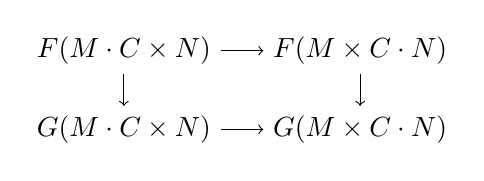
\begin{tikzpicture}
	\node (LT) at (0, 1) {$F(M \cdot C \times N)$};
	\node (LB) at (0, 0) {$G(M \cdot C \times N)$};
	\node (RT) at (3, 1) {$F(M \times C \cdot N)$};
	\node (RB) at (3, 0) {$G(M \times C \cdot N)$};
	\draw [->] (LT) -- node [left] {$$} (LB);
	\draw [->] (LT) -- node [above] {$$} (RT);
	\draw [->] (RT) -- node [right] {$$} (RB);
	\draw [->] (LB) -- node [below] {$$} (RB);
	%\node at (0.5, 1) {$\ulcorner$};
	%\node at (1.5, 0.5) {$\lrcorner$};
\end{tikzpicture}.
\end{center}
\nid Here $M \cdot C$ stands for $\otimes^{\cM}(M \times C)$ and $C \cdot N$ stands for $\otimes^{\cN}(C \times N)$.
\end{definition}


\begin{definition}
	Let $\cA$ and $\cB$ be right and left $\cC$-module categories, respectively. The {\em Deligne tensor product $\cA \boxtimes_{\cC} \cB$} is the universal linear category admitting a $\cC$-balanced multilinear functor $\boxtimes_{\cC}: \cA \times \cB \to \cA \boxtimes_{\cC} \cB$. That is, there exists a $\cC$-balanced multilinear functor $\boxtimes_{\cC}: \cA \times \cB \to \cA \boxtimes_{\cC} \cB$ which induces, for all linear categories $\cD$, an equivalence between the category of $\cC$-balanced multilinear functors $\cA \times \cB \to \cD$ and the category of linear functors $\cA \boxtimes_{\cC} \cB \to \cD$. 
\end{definition}

If it exists, the Deligne tensor product is unique up to an equivalence, which in turn is unique up to unique natural isomorphism. Equivalently, the 2-category of linear categories representing the Deligne tensor product is either contractible or empty. 

\begin{theorem} \label{thm:DelignePrdtOverATCExists}
	Let $\cC$ be a finite tensor category and let $\cA_{\cC}$ and ${}_{\cC}\cB$ be finite right and left $\cC$-module categories, respectively. Then, \CD{Ref to the literature for this theorem?}
	\begin{enumerate}
		\item The Deligne tensor product $\cA \boxtimes_{\cC} \cB$ exists and is a finite linear category;
		\item If $\cA = \Mod{A}{}(\cC)$ and $\cB = \Mod{}{B}(\cC)$, then $\cA \boxtimes_{\cC} \cB \simeq \Mod{A }{B}(\cC)$;
	\end{enumerate} 
%Moreover if $\cC$ is rigid, then 	
%	\begin{enumerate}
%		\item[(3)] The functor $\boxtimes_{\cC}$ is exact in each variable and satisfies 
%		\begin{equation*}
%			\Hom_{\cA}(x,x') \otimes \Hom_{\cB}(y, y') \cong \Hom_{\cA \boxtimes_{\cC} \cB} (x \boxtimes_{\cC} y, x' \boxtimes_{\cC} y'),
%		\end{equation*}
%		\item[(4)] If $F: \cA \times \cB \to \cD$ is a $\cC$-balanced multilinear functor which is exact in each variable, then it defines an exact functor $\overline{F}: \cA \boxtimes_{\cC} \cB \to \cD$. 
%	\end{enumerate} 
\end{theorem}

\begin{proof}
	When $\cC = \Vect_k$, this is classical \cite[Prop 5.13]{MR1106898} (see also \cite[Prop 1.46.2]{EGNO}), and the product $\cA \boxtimes_{\Vect_k} \cB$ is simply denoted $\cA \boxtimes \cB$.
	By Theorem \ref{thm:EGNO2.11.6} to show (1) and (2) it is enough to assume that $\cA = \Mod{A}{}(\cC)$ and $\cB = \Mod{}{B}(\cC)$ and show that $\Mod{A }{B}(\cC)$ has the desired universal property. Tensoring a left $A$-module and a right $B$-module gives a canonical $\cC$-balanced multilinear functor 
		\begin{equation*}
			T: \Mod{A}{}(\cC) \times \Mod{}{B}(\cC) \to \Mod{A}{B}(\cC),  
		\end{equation*}
and we will show that $T$ induces an equivalence between $\cC$-balanced multilinear functors $\cA \times \cB \to \cD$ and linear functors from $\Mod{A}{B}(\cC)$ to $\cD$.
	
	To this end, let $F:\Mod{}{A}(\cC) \times \Mod{B}{}(\cC) \to \cD$ be a $\cC$-balanced multilinear functor.  \CD{The side on which A and B are acting just switched.}
	There is a unique right exact linear functor $\overline F: \Mod{B}{A}(\cC) \to \cA$ such that $F = \overline{F} \circ T$ which is defined as follows. On free bimodules, that is those of the form $A \otimes W \otimes B$ for $W \in \cC$, we have $\overline{F}(A \otimes W \otimes B) \cong F((A \otimes W) \times B)$. Since  every $A$-$B$-bimodule $X$ is a coequalizer of free $A$-$B$-bimodules, namely the canonical coequalizer  
	\begin{equation*}
		X \leftarrow A \otimes X \otimes B \leftleftarrows A \otimes A \otimes X \otimes B \otimes B,
	\end{equation*}
	and since $\overline{F}$ is meant to be right exact, the coequalizer diagram
	\begin{equation*}
		\overline{F}(X) \leftarrow F((A \otimes X) \times B) \leftleftarrows F((A \otimes A \otimes X \otimes B) \times B)
	\end{equation*}
specifies $\overline{F}$ on any bimodule.
%	
%	If $\cC$ is rigid, then by Lemma \ref{lma:RigidIsExact} the functor $T = \boxtimes_{\cC}$ is exact in each variable. The formula in (3) then follows as a standard exercise in using duals. Finally let $F: \cA \times \cB \to \cD$ be a $\cC$-balanced multilinear functor which is exact in each variable and let $\overline{F}: \cA \boxtimes_\cC \cB \to \cD$ be its linear extension (which is always right exact). Since $F$ is exact in each variable, $\overline{F}$ preserves left exact sequences of free $A$-$B$-bimodules (where the maps are also free). Since every $A$-$B$-bimodule has a functorial resolution by free $A$-$B$-bimodules (coming from the above mentioned coequalizer), a diagram chase shows that $\overline{F}$ is also left exact. Hence (4) is also satisfied. 
\end{proof}


%\begin{proposition}[]
%	Let $\cA$ and $\cB$ be finite linear categories. Then,
%	\begin{enumerate}
%		\item The Deligne tensor product $\cA \boxtimes \cB$ exists and is a finite linear category;
%		\item If $\cA = \Mod{A}{}$ and $\cB = \Mod{B}{}$, then $\cA \boxtimes \cB \simeq \Mod{A \otimes B}{}$;
%		\item The functor $\boxtimes$ is exact in each variable and satisfies 
%		\begin{equation*}
%			\Hom_{\cA}(x,x') \otimes \Hom_{\cB}(y, y') \cong \Hom_{\cA \boxtimes \cB} (x \boxtimes y, x' \boxtimes y'),
%		\end{equation*}
%		\item If $F: \cA \times \cB \to \cC$ is a multilinear functor which is exact in each variable, then it defines an exact functor $\overline{F}: \cA \boxtimes \cB \to \cC$. 
%	\end{enumerate} 
%\end{proposition}


\begin{remark} \label{rmk:rigidpreservedbytensor}
	We may rewrite the data  of a tensor category as a linear category $\cD$ equipped with an object $1 \in \cD$ and a linear functor $\otimes: \cD \boxtimes \cD \to \cD $, together with natural transformations $\alpha$, $\lambda$, and $\rho$, satisfying appropriate coherence relations. % Moreover by Corollary \ref{cor:RigidityViaFunctors} the tensor product of two rigid tensor categories is again rigid. 
\end{remark}

\begin{remark}
	If ${}_{\cD}\cA_{\cC}$ and ${}_{\cC}\cB_{\cE}$ are bimodule categories, then the actions of $\cD$ and $\cE$ induce a $\cD$-$\cE$-bimodule category structure on $\cA \boxtimes_{\cC} \cB$. This bimodule category satisfies the analogous universal property for $\cC$-balanced twisted bilinear bimodule functors. 
\end{remark}

\begin{lemma} \label{Lma:FunctorsAsATensorPdt}
	If $\cC$ is a finite tensor category and $\cM$ and $\cN$ are finite left $\cC$-module categories then the natural functor induces an equivalence of linear categories
	\begin{equation*}
		\Fun_\cC(\cM, \cC) \boxtimes_\cC \cN \simeq \Fun_\cC(\cM,\cN).
	\end{equation*} \CD{Need to know that the equivalences is right exact??}
	Here $\Fun_\cC$ denotes the category of (right exact) $\cC$-module functors. 
	Moreover, if $\cM$ and $\cN$ are bimodule categories, then the above equivalence is a bimodule equivalence. 
\end{lemma}

\begin{proof}
	The last sentence follows since in that case the natural functor is a bimodule functor. By Theorem \ref{thm:EGNO2.11.6}, there exist algebra objects $A, B \in \cC$ and equivalences $\cM \simeq \Mod{}{A}(\cC)$ and $\cN \simeq \Mod{}{B}(\cC)$. We show that both sides of the above equation are naturally equivalent to $\Mod{A}{B}(\cC)$, the category of $A$-$B$-bimodule objects in $\cC$. The equivalence $\Fun_\cC(\cM, \cN) \simeq \Mod{A}{B}(\cC)$ (\cite[Prop 2.12.2]{EGNO}) can be seen by mirroring the classical proof, as follows. A bimodule certainly gives rise to such a functor, \CD{Need to define the functor associated to a bimodule for clarity}
	and given a functor $f: \cM \rightarrow \cN$, we obtain an $A$-$B$-bimodule $f(A)$ using the fact that $f$ is a left $\cC$-module functor.  The functor $f$ is equivalent to the one determined by the bimodule $f(A)$: by $\cC$-linearity the functor $f$ is as desired on free $\cA$-modules, namely $f(X \otimes A) \cong X \otimes f(A)  \cong (X \otimes A) \otimes_A f(A)$, and every object of $\cM$ may be written as a (canonical) coequalizer of free $A$-modules,
	\begin{equation*}
		M \leftarrow M \otimes A \leftleftarrows M \otimes A \otimes A.
	\end{equation*} 
Thus the natural map  $\Mod{A}{B}(\cC) \to \Fun_\cC(\cM, \cN)$ is essentially surjective. The above argument also shows it is fully faithful, so that $\Fun_\cC(\cM, \cN) \simeq \Mod{A}{B}(\cC)$, which in particular shows $\Fun_\cC(\cM, \cC) \simeq \Mod{}{A}(\cC)$. Now the result follows from Theorem \ref{thm:DelignePrdtOverATCExists}.
%Tensoring a left $A$-module and a right $B$-module gives a canonical $\cC$-balanced bilinear functor 
%\begin{equation*}
%	T: \Mod{A}{}(\cC) \times \Mod{}{B}(\cC) \to \Mod{A}{B}(\cC). 
%\end{equation*}
%To complete the proof we must show this induces an equivalence,
%\begin{equation*}
%	\Mod{}{A}(\cC) \boxtimes_\cC \Mod{B}{}(\cC) \simeq \Mod{B}{A}(\cC).
%\end{equation*}
%When $\cC = \Vect$, this is classical. More generally we must show that the right-hand-side has the desired universal property. For this purpose let $F:\Mod{}{A}(\cC) \times \Mod{B}{}(\cC) \to \cA$ be a $\cC$-balanced bilinear functor. There is a unique right exact linear functor $\overline F: \Mod{B}{A}(\cC) \to \cA$ such that $F = \overline{F} \circ T$ which is defined as follows. On free bimodules $A \otimes X \otimes B \cong T(A \otimes X, B)$, we necessarily have $\overline{F}(A \otimes X \otimes B) \cong F(A \otimes X, B)$. Since $\overline{F}$ is right exact and every $A$-$B$-bimodule is a coequalizer of free $A$-$B$-bimodules, the result follows. 	
\end{proof} \CD{I think we'll be able to rewrite this proof in a more structured way that makes the logic clearer.}

\begin{remark} \label{remark-tensorasfunctors}
If $\cM$ and $\cN$ are right $\cD$-modules, then we have $\cN \boxtimes_\cD \Fun_{\cD}(\cM,\cD) \simeq \Fun_{\cD}(\cM,\cN)$, and again if $\cM$ and $\cN$ are bimodule categories, then this equivalence is a bimodule equivalence. 
\end{remark}






\section{The symmetric monoidal Segal 3-category of tensor categories} \label{sec-tc-threecat}

\CDcomm{I think the exposition in this section needs reworking, though I don't think it will be too hard.  The issue at the moment is that it is easy for the reader to get confused about which parts of the story are moral and which are actual.  (Eg, first it says ``we will build a functor", then ``one fails to produce a strict functor", then ``this gives a strict functor".)  I think everything `moral' should be in carefully delineated remarks, and the main text should be crystal clear about exactly what is being constructed.  In particular it should be in blinking lights that the functor being produced is a strict functor into a 1-category, and which 1-category should be completely explicit.  Then in the moral remark, it should also be clearer what the moral story is, eg of a weak functor into (specify exactly which 3-category and what kind of 3-category).  (One among various sticky points: the intermediate reader could easily think ``length-n strings of composable bimodule categories" was implicitly meant to include choices of compositions, in order to facillitate forgetful functors, and that ``functors" in the next line means ``weak functors", and indeed has been prepared to think these things---but that is exactly not the point that is being made in the moral paragraphs.)}

We now describe the symmetric monoidal 3-fold Segal category $\TCfin$ of finite tensor categories, finite bimodule categories, linear bimodule functors, and linear bimodule natural transformations. We first construct a functor from $(\Gamma \times \Delta)^\textrm{op}$ to strict 2-categories, such that the Segal maps are equivalences. We may obtain a $\Gamma$-3-fold simplicial space by applying the 2-nerve levelwise.  \CD{Indicate this produces a $\Gamma$-3-fold simplicial \emph{set}.} Lemma \ref{lma:2catnervereflectsequiv} implies that the result is indeed a symmetric monoidal  Segal 3-category.  \CD{That this is the point of that Lemma should be explained in detail back at that Lemma, perhaps as an explicit corollary, whose proof should at least briefly address all the issues, ie Reedy fibrancy, and conditions (1), (2), and (3).}

Let $A$ be a finite set and let $[n]$ be an object of $\Delta$. The strict 2-category $\TCfin(A,n)$ should morally be regarded as the 2-category consisting of $A$-tuples of length-$n$ strings of composable bimodule categories. In other words, if one had a pre-existing notion of 3-category, then $\TCfin(A,n)$ should be thought of as \CDcomm{(what kind of)} functors from the category $A \times [n]$ into the weak 3-category $\TCfin$.

As we have seen, the problem with implementing this straightforward idea is that one fails to produce a {\em strict} functor from $(\Gamma \times \Delta)^\textrm{op}$ to strict $2$-categories. This is due to the fact that both the symmetric tensor product and the composition of bimodule categories are defined via universal properties and are not strictly associative. Thus $\TCfin(A,n)$ consists of an enlarged version which includes, in addition to the 
$A$-tuples of length-$n$ strings of composable bimodule categories, choices of all the possible composites and tensor products that naturally arise. The most canonical way to do this is to define $\TCfin(A,n)$ to include all such possible choices. 


%will have objects which consist of collections of several tensor categories, bimodule categories, functors, and natural transformations which are required to satisfy a host of conditions. The 1- and 2-morphisms of $\TC(A,n)$ will be defined similarly. 

% This is largely due to the fact that  composition of bimodule categories is only weakly defined. It is defined up to equivalence of bimodule categories which are in turn defined up to unique natural isomorphism, but this is not sufficient to obtain a {\em strict} functor on $(\Gamma \times \Delta)^\textrm{op}$. One solution is to enlarge $\TC(A,n)$ to include choices of all the possible composites that one would need in order to obtain a strict functor to strict 2-categories. The resulting $\TC(A,n)$ is what we now describe.


 Thus the objects of $\TCfin(A,n)$ are certain compatible collections of finite tensor categories, finite bimodule categories, and their various maps. \CD{their various maps?} These collections are parametrized by certain $k$-faces of the simplex $[n]$ and collections of disjoint subsets of $A$. We summarize the data of an object $X \in \TCfin(A,n)$ in Tables \ref{Table:ObjectOfTC} and \ref{Table:ObjectOfTC2}. \CD{Combine tables 1 and 2 into a single table, as with table 3.} \CD{In table 2, ``$(X_{S;j} \times X_{S;k})$-balanced"?, or explain the use of $X_{S;j} / X_{S;k}$.}
\begin{table}[ht]
	\caption{Data and Conditions for an object of $\TCfin(A,n)$.}
	\begin{tabular}{c |ccccc}
	 subsets \textbackslash\ faces & vertex $i$ & edge $ij$ & 2-face $ijk$ & 3-face $ijk\ell$ & 4-face \\
	\hline
	$S$ 				& $X_{S;i}$ & $X_{S; ij}$ & $b_{S; ijk}$  & $\alpha_{S;ijk\ell}$ & (TCO3) \\
	$S, S'$ 			& $x_{S, S';i}$ & $x_{S, S';ij}$ & $\psi_{S, S'; i j k}$ & (TCO4) & \\
	$S, S', S''$ 		& $\alpha_{S, S', S'';i}$ & $\alpha_{S, S', S'';ij}$ & (TCO5) &  & \\
	\hline
	$S, S', S'', S''' $	& \multicolumn{2}{c}{ \begin{tikzpicture}[baseline=-0.1cm]\draw [->] (0,0) -| (-0.2, 0.15);\end{tikzpicture} (TCO6) \begin{tikzpicture}[baseline=-0.1cm]\draw [->] (0,0) -| (0.2, 0.15);\end{tikzpicture} } &  &  & \\
	\end{tabular}
	\label{Table:ObjectOfTC}
\end{table}	
\begin{table}[ht]
	\caption{Description of the Data of an object of $\TCfin(A,n)$.}	
	\begin{tabular}{l p{11cm}}
		datum & description of datum \\ \hline
		$X_{S;i}$ & A finite tensor category \\
		$X_{S;ij}$ & An finite $X_{S;i}$-$X_{S,j}$-bimodule category. \\
		$b_{S; ijk}$ & An $X_{S;j}$-balanced $X_{S;i}$-$X_{S,k}$-bilinear functor from $X_{S;ij}\times X_{S;jk}$ to $X_{S;ik}$. \\
		$\alpha_{S;ijk \ell}$  & A natural isomorphism of $X_{S;j}$/$X_{S;k}$-balanced $X_{S'i}$-$X_{S;\ell}$-bimodule functors from $b_{S;i k \ell} \circ (b_{S;ijk} \times id_{X_{S;k\ell}})$ to $b_{S;ij \ell} \circ (id_{X_{S;ij}} \times b_{S;jk\ell})$. \\ \hline
		$x_{S, S';i}$ & A bilinear tensor functor from $X_{S;i} \times X_{S';i}$ to $X_{S \cup S'; i}$. \\
		$x_{S, S';ij}$ & A twisted bilinear bimodule functor from $X_{S;ij} \times X_{S';ij}$ to $X_{S \cup S'; ij}$, extending $x_{S, S';i}$ and $x_{S, S';j}$. \\
		$\psi_{S, S'; i j k}$ & A natural isomorphism of $X_{S;j} / X_{S';j}$-balanced bimodule functors from $x_{S,S'; ik} \circ (b_{S; ijk} \times b_{S';ijk})$ to $b_{S \cup S'; ijk} \circ (x_{S,S';ij} \times x_{S \cup S'; jk}) \circ  \tau $, where $\tau$ exchanges the middle two factors.  \\ \hline
		$\alpha_{S, S', S'';i}$ & A natural isomorphism of multilinear tensor functors from
		$x_{S \sqcup S', S'';i}\circ (x_{S,S';i} \times 1)$  to 
		$x_{S, S' \sqcup S'';i} \circ (1 \times x_{S', S'';i})$. \\
		$\alpha_{S, S', S'';ij}$ & A natural isomorphism of multilinear bimodule functors from
		$x_{S \sqcup S', S'';ij}\circ (x_{S,S';ij} \times 1)$  to 
		$x_{S, S' \sqcup S'';ij} \circ (1 \times x_{S', S'';ij})$. \\
	\end{tabular}
	\label{Table:ObjectOfTC2}
\end{table}
This data is required to satisfy the following conditions: \\
\newcounter{itemcounter}
\begin{list}{(TCO\arabic{itemcounter})}{\usecounter{itemcounter}}
%	\setlength{\leftmargin}{0pt}
	\item  The functors $x_{S,S';i}$, $x_{S,S'; ij}$, and $b_{S;ijk}$ realize equivalences with the following Deligne tensor products:
	\begin{align*}
		X_{S \cup S'; i} &\cong X_{S; i} \boxtimes X_{S';i} \\ 
		X_{S \cup S'; ij} &\cong X_{S; ij} \boxtimes X_{S';ij} \\ 
		X_{S; ik} & \cong X_{S;ij} \boxtimes_{X_{S;j}} X_{S;jk}
	\end{align*}
	\item  $X_{\emptyset; i} \cong \Vect$, with $X_{\emptyset; ij}$, $b_{\emptyset; ijk}$, and $\alpha_{\emptyset; ijk\ell}$ respectively the identity bimodule category, the tensor functor, and the tensor associator.  Moreover when either $S$ or $S'$ is empty, the functors $x_{S,S'; i}$ and $x_{S, S'; ij}$ and the transformation $\psi_{S,S'; ijk}$ are the canonical ones.  \CD{Is the iso of $X_{\emptyset;i}$ and $\Vect$ chosen?  If not, then I don't know what the morphism $X_{S,\emptyset;i}$ is.  And even if the iso is chosen, the $\Vect$ action needs to be constructed somewhere, right?  (Just because it's unique up to iso isn't good enough at this moment, right?)}
	\item  For every $S$ and every 4-simplex $ijk\ell m$, the isomorphisms $\alpha_{S; -}$ satisfy the appropriate pentagon equation.

	\item  For every pair of disjoint subsets $S, S'$ and every 3-simplex $ijk\ell$, the `hexagon' equation in Figure \ref{fig:EqnSSijkObject} is satisfied. 
\begin{figure}[ht]
	\caption{Equation for condition (TCO4) on the data of an object of $\TCfin(A,n)$.}
	\begin{center}
		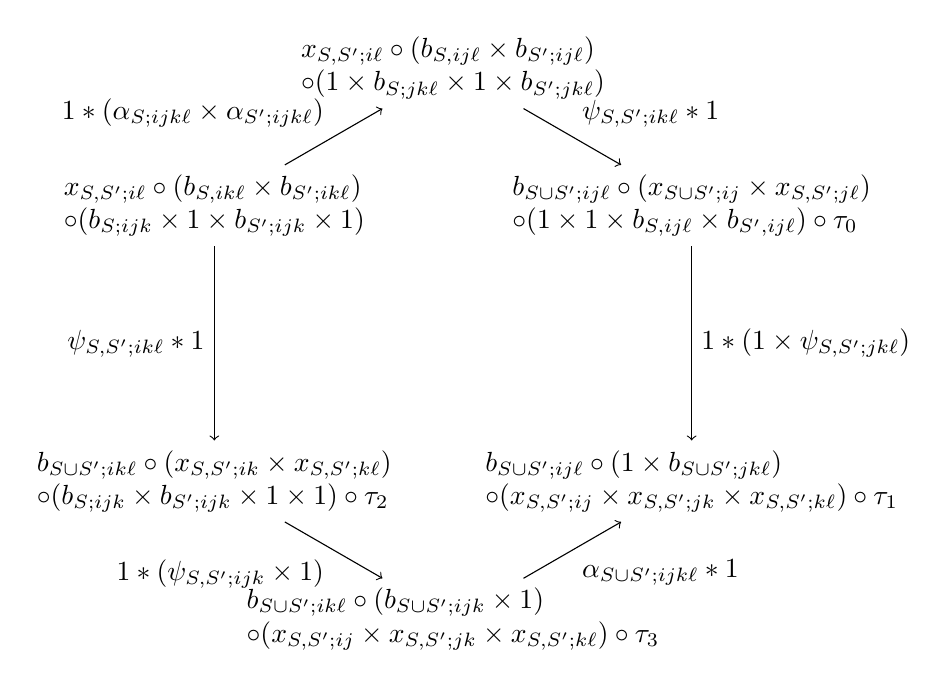
\begin{tikzpicture}[align=left]
	%		\node (A) at (126:2cm) {A};
	%		\node (B) at (54:2cm) {B};
	%		\node (C) at (342:2cm) {C}; % -18 degrees
	%		\node (D) at (270:2cm) {D};
	%		\node (E) at (198:2cm) {E};		
			\node  (A) at (150:3.5cm) {$x_{S, S'; i\ell} \circ (b_{S, ik\ell} \times b_{S'; ik\ell})$ \\ $\circ (b_{S; ijk} \times 1 \times b_{S'; ijk} \times 1)$};
			\node (B) at (90:3.5cm) {$x_{S, S'; i\ell} \circ (b_{S, ij\ell} \times b_{S'; ij\ell})$\\ $ \circ (1 \times b_{S; jk\ell} \times 1 \times b_{S'; jk\ell})$};
			\node (C) at (30:3.5cm) {$b_{S\cup S'; ij\ell} \circ (x_{S\cup S'; ij} \times x_{S, S'; j\ell}) $\\ $ \circ (1 \times 1 \times b_{S, ij\ell} \times b_{S', ij\ell} ) \circ \tau_0$}; 
			\node (D) at (330:3.5cm) {$b_{S\cup S'; ij\ell} \circ (1 \times b_{S \cup S'; jk\ell}) $\\ $ \circ (x_{S, S'; ij} \times x_{S, S'; jk} \times x_{S, S'; k\ell}) \circ \tau_1$};
			\node (E) at (270:3.5cm) {$b_{S \cup S'; ik\ell} \circ (b_{S \cup S';ijk} \times 1) $\\$ \circ (x_{S, S'; ij} \times x_{S, S'; jk} \times x_{S, S'; k\ell}) \circ \tau_3$};
			\node (F) at (210:3.5cm) {$b_{S \cup S'; ik\ell} \circ (x_{S, S'; ik} \times x_{S, S'; k \ell}) $\\$ \circ (b_{S;ijk} \times b_{S';ijk} \times 1 \times 1) \circ \tau_2$};
			\draw [->] (A) to node [above left] {$1*(\alpha_{S; ijk\ell} \times \alpha_{S'; ijk\ell})$} (B);
			\draw [->] (B) to node [above right] {$\psi_{S, S'; ik\ell}*1$} (C);
			\draw [->] (C) to node [right] {$1 * (1 \times \psi_{S,S'; jk\ell})$} (D);
			\draw [->] (A) to node [left] {$\psi_{S, S'; ik\ell}*1$} (F);
			\draw [->] (F) to node [below left] {$1 * (\psi_{S,S'; ijk} \times 1)$} (E);
			\draw [->] (E) to node [below right] {$\alpha_{S \cup S';ijk\ell} * 1$} (D);
		\end{tikzpicture}
	\end{center}
	\label{fig:EqnSSijkObject}
\end{figure} \CD{CD has not checked Figures 1, 2, 3, 4, 5, nor TC2M1, TC2M2.}
There, each $\tau_i$ represents an appropriate permutation of the factors. In other words, $(x_{S,S';-}, \psi_{S, S'; -})$ forms a structure analogous to a functor of bicategories. \CD{Omit the sentence beginning ``In other words"?}
	\item  For every triple of disjoint subsets $S, S', S''$ and every 2-simplex $ijk$, the  `hexagon' equation in Figure \ref{fig:EqnSSSijObject} holds.
	\begin{figure}[ht]
		\caption{Equation for condition (TCO5) on the data of an object of $\TCfin(A,n)$.}
	\begin{center}
		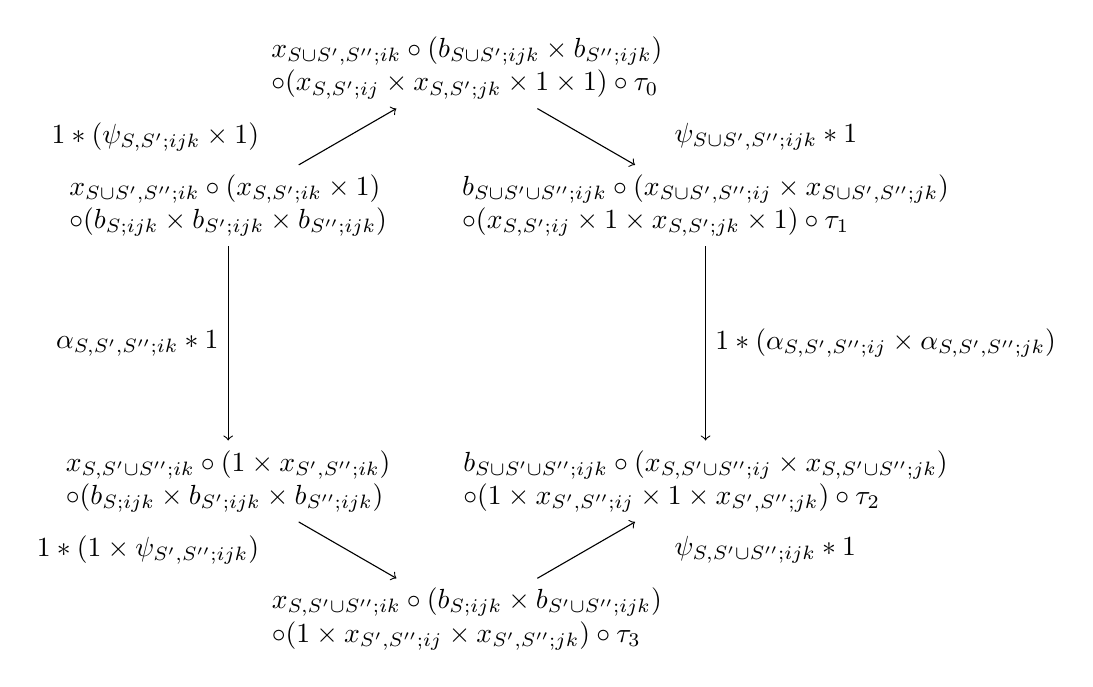
\begin{tikzpicture}[align=left]
	%		\node (A) at (126:2cm) {A};
	%		\node (B) at (54:2cm) {B};
	%		\node (C) at (342:2cm) {C}; % -18 degrees
	%		\node (D) at (270:2cm) {D};
	%		\node (E) at (198:2cm) {E};		
			\node (A) at (150:3.5cm) {$x_{S \cup S', S'';ik} \circ (x_{S, S'; ik} \times 1) $\\$\circ (b_{S;ijk} \times b_{S';ijk} \times b_{S'';ijk})$};
			\node (B) at (90:3.5cm) {$x_{S \cup S', S'';ik} \circ (b_{S\cup S'; ijk} \times b_{S''; ijk}) $\\$ \circ (x_{S, S'; ij} \times x_{S, S'; jk} \times 1 \times 1) \circ \tau_0$};
			\node (C) at (30:3.5cm) {$b_{S \cup S' \cup S''; ijk} \circ (x_{S \cup S', S''; ij} \times x_{S \cup S', S''; jk}) $\\$ \circ (x_{S, S'; ij} \times 1 \times x_{S, S'; jk} \times 1 ) \circ \tau_1$}; 
			\node (D) at (330:3.5cm) {$b_{S \cup S' \cup S''; ijk} \circ (x_{S , S' \cup S''; ij} \times x_{S,  S'\cup S''; jk}) $\\$ \circ ( 1 \times x_{S', S''; ij} \times 1 \times x_{S', S''; jk}) \circ \tau_2$};
			\node (E) at (270:3.5cm) {$x_{S, S' \cup S'';ik} \circ (b_{S;ijk} \times b_{S' \cup S''; ijk}) $\\$ \circ (1 \times x_{S', S'';ij} \times x_{S', S''; jk})  \circ \tau_3$};
			\node (F) at (210:3.5cm) {$x_{S, S' \cup S'';ik} \circ (1 \times x_{S', S''; ik} ) $\\$ \circ (b_{S;ijk} \times b_{S';ijk} \times b_{S'';ijk})$};
			\draw [->] (A) to node [left=1cm] {$1* (\psi_{S, S';ijk}\times 1)$} (B);
			\draw [->] (B) to node [right=1cm] {$\psi_{S\cup S', S''; ijk} * 1$} (C);
			\draw [->] (C) to node [right] {$1 * (\alpha_{S,S',S''; ij} \times \alpha_{S, S', S''; jk})$} (D);
			\draw [->] (A) to node [left] {$\alpha_{S, S', S'';ik}*1$} (F);
			\draw [->] (F) to node [ left=1cm] {$1 * (1 \times \psi_{S', S''; ijk})$} (E);
			\draw [->] (E) to node [right=1cm] {$\psi_{S, S' \cup S''; ijk}*1$} (D);
		\end{tikzpicture}
	\end{center}
		\label{fig:EqnSSSijObject}
	\end{figure}
	There, $\tau_i$ is an appropriate permutation of the factors. 
	\item  For every quadruple of disjoint subsets $S, S', S'', S'''$, the isomorphisms $\alpha_{-; i}$ and $\alpha_{-; ij}$ satisfy the appropriate pentagon equations. When $S' = \emptyset$ then $\alpha_{S, S', S''; i}$ and $\alpha_{S, S', S''; ij}$ satisfy the appropriate triangle identity. \CD{You are sure the identities for $S = \emptyset$ and $S'' = \emptyset$ follow (as classically)?} 
\end{list}

Let $X$ and $Y$ be two objects in $\TCfin(A,n)$. A 1-morphism from $X$ to $Y$ may only exist if each of the tensor categories agree identically $X_{S;i} = Y_{S;i}$ for each subset $S \subseteq A$ and vertex $i$ of $[n]$. \CD{Why not allow tensor functors here, so $F_{S;ij}$ become twisted bimodule functors? (`Because it makes everything harder' might be an answer, but I was surprised by the restriction.)}
In this case the 1-morphisms from $X$ to $Y$ consist of collections of data as in Table \ref{Table:1MorOfTC}.
\begin{table}[h]
	\caption{Data of a 1-morphism of $\TCfin(A,n)$.}
	\begin{tabular}{c |cccc}
	 subsets \textbackslash\ faces & vertex $i$ & edge $ij$ & 2-simplex $ijk$ & 3-simplex $ijk\ell$  \\
	\hline
	$S$ 				& n/a & $F_{S; ij}$ & $\xi_{S; ijk}$  &  (TC1M2) \\
	$S, S'$ 			& n/a & $\varphi_{S, S';ij}$ &  (TC1M3) & \\
	$S, S', S''$ 		& n/a  & (TC1M4) & & \\
	\end{tabular}
	
	\vspace{0.5cm}
	
	\begin{tabular}{l p{11cm}}
		datum & description of datum \\ \hline
		$F_{S;ij}$ & An $X_{S;i}$-$X_{S;j}$-bimodule functor from $X_{S;ij}$ to $Y_{S;ij}$. \\
		$\xi_{S;ijk}$ & A natural isomorphism of $X_{S;j}$-balanced $X_{S;i}$-$X_{S;k}$-bimodule functors from $b^Y_{S;ijk} \circ (F_{S;ij} \times F_{S; jk})$ to $F_{S;ik} \circ b^X_{S;ijk}$. \\
		$\varphi_{S,S'; ij}$ & A natural isomorphism of bilinear bimodule functors from $y_{S,S'; ij} \circ (F_{S; ij} \times F_{S';ij})$ to $F_{S \cup S'; ij} \circ x_{S, S'; ij}$. 
	\end{tabular}
	\label{Table:1MorOfTC}
\end{table}
This data is required to satisfy the following axioms:
\begin{list}{(TC1M\arabic{itemcounter})}{\usecounter{itemcounter}}
	\item If $S = \emptyset$, then $F_{S;ij}$ and $\xi_{S;ijk}$ are identities. If either $S$ or $S'$ is equal to $\emptyset$, then $\varphi_{S,S';ij}$ is the canonical map.  \CD{Re TC1M1: As (TCO2) is written, there aren't identities here to ask for.  Also, I haven't checked if there is actually a canonical map.}
	\item For every subset $S$ and every 3-simplex $ijk\ell$ the hexagon equation in Figure \ref{fig:EqnSijklMorphism} holds.
	\begin{figure}[ht]
		\caption{Equation for condition (TC1M2) on the data of a 1-morphism of $\TCfin(A,n)$.}
		\begin{center}
			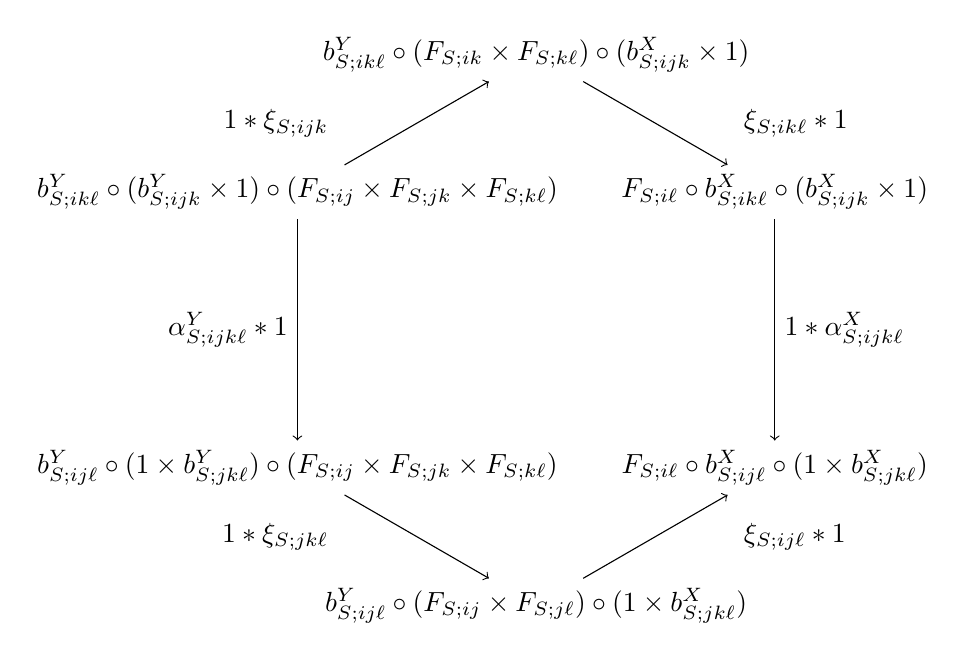
\begin{tikzpicture}[align=left]	
				\node (A) at (150:3.5cm) {$b^Y_{S;ik\ell} \circ (b^Y_{S;ijk} \times 1) \circ (F_{S;ij} \times F_{S;jk} \times F_{S;k\ell})$};
				\node (B) at (90:3.5cm) {$b^Y_{S;ik\ell} \circ (F_{S;ik} \times F_{S;k\ell}) \circ (b^X_{S;ijk} \times 1) $};
				\node (C) at (30:3.5cm) {$F_{S;i\ell} \circ b^X_{S;ik\ell} \circ (b^X_{S;ijk} \times 1)$}; 
				\node (D) at (330:3.5cm) {$F_{S;i\ell} \circ b^X_{S;ij\ell} \circ (1 \times b^X_{S;jk\ell})$};
				\node (E) at (270:3.5cm) {$b^Y_{S;ij\ell} \circ (F_{S;ij} \times F_{S;j\ell}) \circ (1 \times b^X_{S;jk\ell}) $};
				\node (F) at (210:3.5cm) {$b^Y_{S;ij\ell} \circ (1 \times b^Y_{S;jk\ell})  \circ (F_{S;ij} \times F_{S;jk} \times F_{S;k\ell})$};
				\draw [->] (A) to node [left=1cm] {$1*\xi_{S;ijk}$} (B);
				\draw [->] (B) to node [right=1cm] {$\xi_{S; ik\ell} * 1$} (C);
				\draw [->] (C) to node [right] {$1*\alpha^X_{S;ijk\ell}$} (D);
				\draw [->] (A) to node [left] {$\alpha^Y_{S;ijk\ell} * 1$} (F);
				\draw [->] (F) to node [ left=1cm] {$1*\xi_{S;jk\ell}$} (E);
				\draw [->] (E) to node [right=1cm] {$\xi_{S; ij\ell}*1$} (D);
			\end{tikzpicture}
		\end{center}
		\label{fig:EqnSijklMorphism}
	\end{figure}
	\item For every pair of disjoint subsets $S, S'$ and every 2-simplex $ijk$ the hexagon equation in Figure \ref{fig:EqnSSijkMorphism} holds, where $\tau$ permutes the middle factors. 
	\begin{figure}[ht]
		\caption{Equation for condition (TC1M3) on the data of a 1-morphism of $\TCfin(A,n)$.}
		\begin{center}
			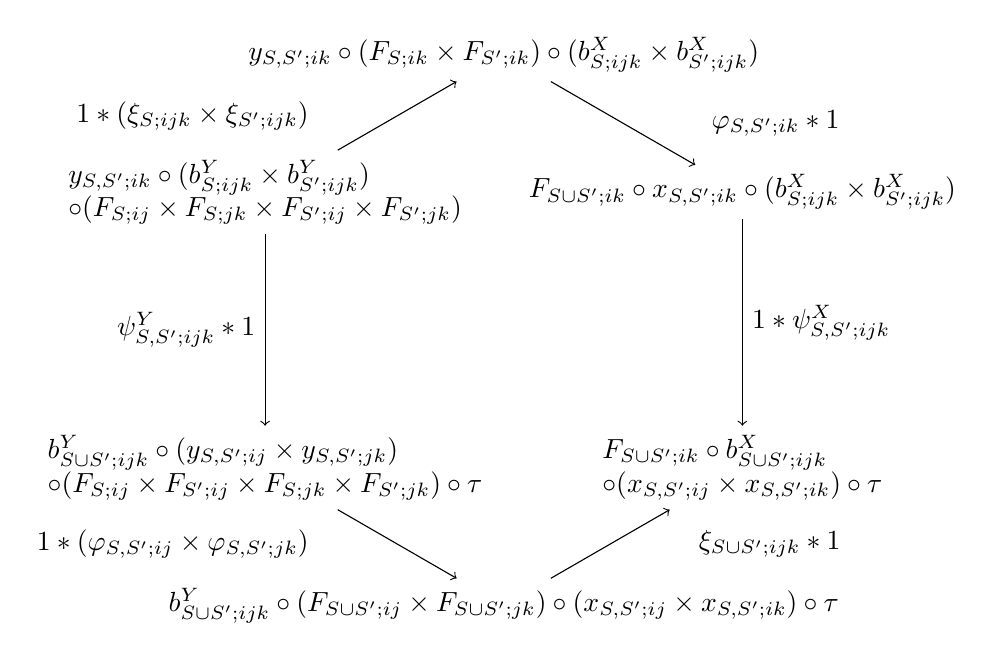
\begin{tikzpicture}[align=left]	
				\node (A) at (150:3.5cm) {$y_{S, S'; ik} \circ (b^Y_{S; ijk} \times b^Y_{S';ijk}) $\\$ \circ (F_{S; ij} \times F_{S; jk} \times F_{S'; ij} \times F_{S'; jk})$};
				\node (B) at (90:3.5cm) {$y_{S, S'; ik} \circ (F_{S; ik} \times F_{S'; ik}) \circ (b^X_{S;ijk} \times b^X_{S'; ijk}) $};
				\node (C) at (30:3.5cm) {$F_{S \cup S'; ik} \circ x_{S, S'; ik} \circ (b^X_{S;ijk} \times b^X_{S'; ijk})$}; 
				\node (D) at (330:3.5cm) {$F_{S \cup S'; ik} \circ b^X_{S \cup S'; ijk} $\\$ \circ (x_{S,S'; ij} \times x_{S,S'; ik}) \circ \tau$};
				\node (E) at (270:3.5cm) {$ b^Y_{S \cup S'; ijk} \circ (F_{S \cup S'; ij} \times F_{S \cup S'; jk}) \circ (x_{S,S'; ij} \times x_{S,S'; ik}) \circ \tau$};
				\node (F) at (210:3.5cm) {$ b^Y_{S \cup S'; ijk} \circ (y_{S,S'; ij} \times y_{S, S'; jk}) $\\$  \circ (F_{S; ij} \times F_{S'; ij} \times F_{S; jk}  \times F_{S'; jk}) \circ \tau$};
				\draw [->] (A) to node [left=1cm] {$1* (\xi_{S;ijk} \times \xi_{S';ijk})$} (B);
				\draw [->] (B) to node [right=1cm] {$\varphi_{S,S';ik}*1$} (C);
				\draw [->] (C) to node [right] {$1* \psi^X_{S, S'; ijk}$} (D);
				\draw [->] (A) to node [left] {$\psi^Y_{S, S'; ijk} * 1$} (F);
				\draw [->] (F) to node [ left=1cm] {$1* (\varphi_{S, S'; ij} \times \varphi_{S, S'; jk})$} (E);
				\draw [->] (E) to node [right=1cm] {$\xi_{S \cup S'; ijk}*1$} (D);
			\end{tikzpicture}
		\end{center}
		\label{fig:EqnSSijkMorphism}
	\end{figure} 
	\item For every triple of disjoint subsets $S, S', S''$ and every edge $ij$, the hexagon equation in Figure \ref{fig:EqnSSSijMorphism} holds.
	\begin{figure}[ht]
		\caption{Equation for condition (TC1M4) on the data of a 1-morphism of $\TCfin(A,n)$.}
		\begin{center}
			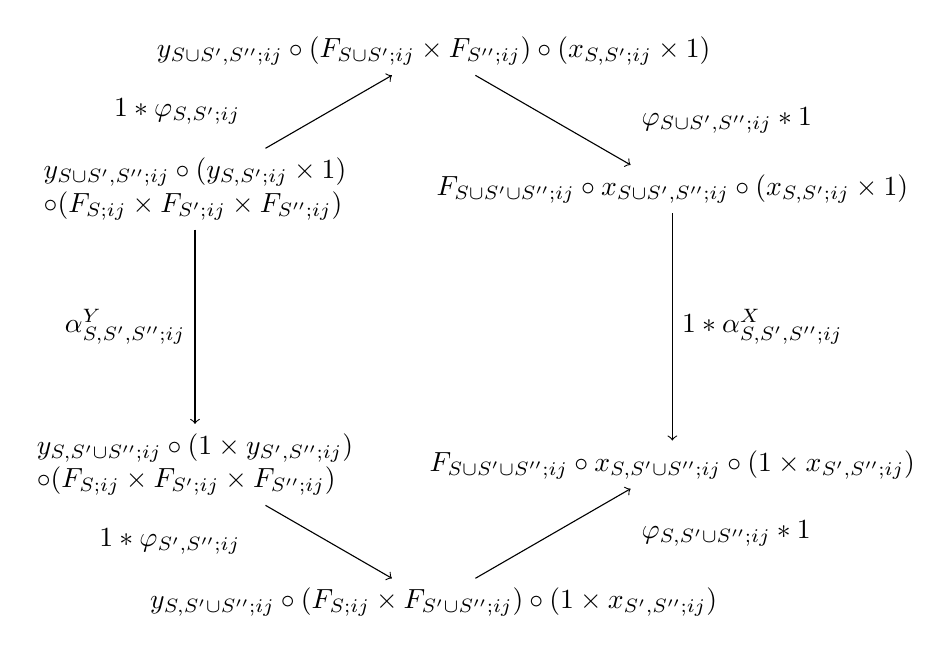
\begin{tikzpicture}[align=left]	
				\node (A) at (150:3.5cm) {$y_{S \cup S', S''; ij} \circ (y_{S, S'; ij} \times 1) $\\$ \circ (F_{S; ij} \times F_{S'; ij} \times F_{S''; ij})$};
				\node (B) at (90:3.5cm) {$y_{S \cup S', S''; ij} \circ (F_{S \cup S'; ij} \times F_{S'';ij}) \circ (x_{S,S';ij} \times 1) $};
				\node (C) at (30:3.5cm) {$F_{S \cup S' \cup S''; ij} \circ x_{S \cup S', S''; ij} \circ (x_{S,S';ij} \times 1)$}; 
				\node (D) at (330:3.5cm) {$F_{S \cup S' \cup S''; ij} \circ x_{S, S'\cup S''; ij} \circ (1 \times x_{S',S'';ij})$};
				\node (E) at (270:3.5cm) {$y_{S,  S'\cup S''; ij} \circ (F_{S;ij} \times F_{S' \cup S''; ij}) \circ (1 \times x_{S', S'';ij}) $};
				\node (F) at (210:3.5cm) {$y_{S,  S'\cup S''; ij} \circ (1 \times y_{S', S''; ij}) $\\$ \circ (F_{S; ij} \times F_{S'; ij} \times F_{S''; ij})$};
				\draw [->] (A) to node [left=1cm] {$1*\varphi_{S,S';ij}$} (B);
				\draw [->] (B) to node [right=1cm] {$\varphi_{S\cup S', S''; ij}*1$} (C);
				\draw [->] (C) to node [right] {$1 * \alpha^X_{S,S', S''; ij}$} (D);
				\draw [->] (A) to node [left] {$\alpha^Y_{S, S', S'';ij}$} (F);
				\draw [->] (F) to node [ left=1cm] {$1 * \varphi_{S', S''; ij}$} (E);
				\draw [->] (E) to node [right=1cm] {$\varphi_{S, S' \cup S''; ij}*1$} (D);
			\end{tikzpicture}
		\end{center}
		\label{fig:EqnSSSijMorphism}
	\end{figure}
\end{list}
A 2-morphism between 1-morphisms $F$ and $G$ from $X$ to $Y$ consists of a collection of $\{ \theta_{S;ij} \}$ consisting of $X_{S;i}$-$X_{S;j}$-bimodule natural transformations from $F_{S;ij}$ to $G_{S;ij}$ for each subset $S \subseteq A$ and 1-simplex $ij$ in $[n]$. For completeness we record this in Table \ref{Table:2MorOfTC}.
\begin{table}[h]
	\caption{Data of a 2-morphism of $\TCfin(A,n)$.}
	\begin{tabular}{c |ccc}
	 subsets \textbackslash\ faces & vertex $i$ & edge $ij$ & 2-simplex $ijk$   \\
	\hline
	$S$ 				& n/a & $\theta_{S; ij}$ &     (TC2M1) \\
	$S, S'$ 			& n/a &  (TC2M2)  &    \\
	\end{tabular}
%	
%	\vspace{0.5cm}
%	
%	\begin{tabular}{l p{11cm}}
%		datum & description of datum \\ \hline
%		$\theta_{S;ij}$ & An $X_{S;i}$-$X_{S;j}$-bimodule natural transformation from $X_{S;ij}$ to $Y_{S;ij}$. 
%	\end{tabular}
	\label{Table:2MorOfTC}
\end{table}
These are required to satisfy that $\theta_{\emptyset;ij}$ is the identity and the following two equations hold:
\begin{list}{(TC2M\arabic{itemcounter})}{\usecounter{itemcounter}}
	\item For each 2-simplex $ijk$, we have
	\begin{equation*}
		(\theta_{S; ik} * 1) \circ \xi^F_{S; ijk} = \xi^G_{S;ijk} \circ (1 * (\theta_{S; ij} \times \theta_{S; jk})).
	\end{equation*}
	\item For each pair of disjoint subsets $S, S'$ we have
	\begin{equation*}
		(\theta_{S \cup S'; ij} * 1) \circ \varphi^F_{S, S'; ij} = \varphi^G_{S,S';ij} \circ (1*(\theta_{S;ij} \times \theta_{S';ij})).
	\end{equation*}
\end{list}
With these as objects, 1-morphisms, and 2-morphisms, the obvious composition makes $\TCfin(A,n)$ into a strict $2$-category.  \CD{Need to specify the three pieces of composite data.}
It is manifestly functorial in $A$ and $[n]$ and thus gives a (strict) functor \CD{CD has not checked that it is a strict 2-category, nor that it is functorial in $A$ and $[n]$.}
\begin{equation*}
	\TCfin: \Gamma^\textrm{op} \times \Delta^\textrm{op} \to 2-\Cat.
\end{equation*}
from the 1-category $\Gamma^\textrm{op} \times \Delta^\textrm{op}$ into the 1-category of strict 2-categories. Composing with the coherent nerve for strict 2-categories gives us a $\Gamma$-3-fold simplicial space, which we also denote $\TCfin$. 

\begin{theorem}
	 $\TCfin$ is a symmetric monoidal Segal 3-category.  
\end{theorem}
\begin{proof}
	Beginning with $\TCfin$,
	by Lemma \ref{lma:2catnervereflectsequiv} it is enough to show that the functor to strict 2-categories satisfies the appropriate Segal conditions, namely that the following Segal maps are weak equivalences of strict 2-categories: \CD{Need to say what a weak equivalence of strict 2-categories is, and what a pullback of strict 2-categories is.  (This might be done earlier.)}
	\begin{align*}
		\TCfin(A, m + n) & \to \TCfin(A, m) \times_{\TCfin(A, 0)} \TCfin(A, n), \\
		\TCfin(A, n) & \to \TCfin(1, n)^{\times |A|}. 
	\end{align*}
In each case the difference between the left-hand-side and the right-hand-side consists of a space of choices of representatives of a Deligne tensor product (and maps representing the tensor product). The category of such choices is contractible (by the universal property of the Deligne tensor product), and so these Segal maps are equivalences, as required. 
\end{proof}

Many variations of this construction are possible. For example if there is a class of tensor categories which is closed under the Deligne tensor product (and contains $\Vect$) or if there is a class of bimodule categories which contains the identities and is closed under composition and tensor product, then we may form restricted versions of $\TC$. In \cite{DSPS} we use this to restrict to the sub-symmetric monoidal Segal 3-categories of rigid tensor categories and module categories satisfying a certain `separability' condition.  \CD{We shouldn't end the paper on an undefined term.}

These techniques may also be adapted to construct other examples of symmetric monoidal Segal $n$-categories. The theory of conformal nets \cite{0912.5307} is another intriguing target for fully local topological field theories. It seems likely, using the work of Bartels-Douglas-Henriques, that the theory of conformal nets may be described as a symmetric monoidal Segal 3-category.  \CD{Think about whether to include or omit this last paragraph, or if included it should be mentioned in the intro rather than here at the end.}

\CD{CD to check that all data of an internal cat in 2Cat has been covered.}
\CD{Discuss whether to reference TC as a cat in 2Cat (BDH).}


\tikzexternalenable


%% The Bibliography
\bibliographystyle{alpha}
\bibliography{bibliography/bibliography}

%\section{Dustbin}


%\begin{definition}
%	A $0$-fold simplicial space (i.e. a simplicial set) is a {\em $0$-fold Segal category} if it is a Kan complex. An $n$-fold simplicial space $X$, regarded as a simplicial object $X_\bullet$ in $(n-1)$-fold simplicial spaces is an {\em $n$-fold Segal category} if the following conditions are satisfied
%		\begin{enumerate}
%			\item The $(n-1)$-fold simplicial space $X_0$ is constant and discrete.
%			\item Each of the $(n-1)$-fold simplicial spaces $X_k$ is an $(n-1)$-fold Segal category.
%			\item For every $m, k$, the Segal square,
%			\begin{center}
%			\begin{tikzpicture}
%				\node (LT) at (0, 1.5) {$X_{m+n}$};
%				\node (LB) at (0, 0) {$X_m$};
%				\node (RT) at (2, 1.5) {$X_n$};
%				\node (RB) at (2, 0) {$X_0$};
%				\draw [->] (LT) -- node [left] {$$} (LB);
%				\draw [->] (LT) -- node [above] {$$} (RT);
%				\draw [->] (RT) -- node [right] {$$} (RB);
%				\draw [->] (LB) -- node [below] {$$} (RB);
%				%\node at (0.5, 1) {$\ulcorner$};
%				%\node at (1.5, 0.5) {$\lrcorner$};
%			\end{tikzpicture}
%			\end{center}
%			is a homotopy pull-back square of $(n-1)$-fold simplical spaces, computed with the $(\infty, n-1)$-model structure.
%		\end{enumerate}
%	\end{definition}
%This final condition requires some explanation. The Segal square must realize $X_{m+n}$ as the homotopy fiber product $X_m \times_{X_0}^h X_n$, and this homotopy fiber product must be computed in the $(\infty, n-1)$-category model structure on $(n-1)$-fold simplicial sets. Moreover $X_{m+n}$ may not be levelwise equivalent to this homotopy fiber product, but merely weakly equivalent in this model structure. Fortunately, we require that $X_0$ is a discrete $(n-1)$-fold simplicial space. In this case the homotopy fiber product simplifies and is merely the ordinary fiber product. Thus condition (3) is equivalent to:
%
%\begin{enumerate}
%	\item [(3')] For every $m$ and $k$ the Segal map $X_{m+n} \to X_m \times_{X_0} X_n$ is an equivalence of $(n-1)$-fold Segal categories. 
%\end{enumerate}
%
%Moreover equivalences between $n$-fold Segal categories admit a fairly tractable inductive recognition principle. To describe this me must introduce a few auxiliary concepts. Let $X$ be an $n$-fold Segal category. Recall that $X_0$ is a constant discrete simplicial space, and so may be regarded as a set.

%
%----
%
%For rigid tensor categories, it will sometimes be convenient to have an alternative description of $\Fun_C(\cM,\cC)$.
%
%\begin{definition}
%Let ${}^*\cM$ denote the $\cD$--$\cC$ bimodule category whose underlying category is $\cM^{\op}$ and the action is given by $d\cdot m \cdot c = {}^*c \otimes m \otimes {}^*d$.  Similarly, let Let $\cM^*$ denote the $\cD$--$\cC$ bimodule category whose underlying category is $\cM^{\op}$ and the action is given by $d\cdot m \cdot c = c^* \otimes m \otimes d^*$.  
%\end{definition}
%
%\begin{lemma}
%If ${}_{\cC}\cM_\cD$ is a $\cC$-$\cD$ bimodule category and ${}_{\cC}\cN_\cE$ is a $\cC$-$\cE$ bimodule category, then taking right adjoints gives an equivalence of $\cD$-$\cE$ bimodules $\Fun_{\cC}(\cM, \cN)$ and ${}^*\Fun^L_{\cC}(\cN, \cM)$ where $\Fun^L_\cC$ denotes \em{left exact} $\Vect$-enriched module functors.  Similarly, if $\cM$ is a $\cC$-$\cD$ bimodule category and $\cN$ is a $\cD$-$\cE$ bimodule category, then taking right adjoints gives an equivalence of $\cC$-$\cE$ bimodules $\Fun_{D}(\cM, \cN) \rightarrow \Fun^L_{\cC}(\cN, \cM)^*$. 
%\end{lemma}
%\begin{proof}
%We've already seen that the adjoint of a module functor has a canonical module functor structure.  Furthermore, taking adjoints is clearly an equivalence because the right adjoint is quasi-inverse to the left adjoint and vice-versa.  So we need only check that the module structures agree.  First note that taking adjoints interchanges precomposition and postcomposition.  Second, in the former case we have that the right adjoint of left multiplication by $x$ is left multiplication by ${}^*x$, while in the latter case we have that the right adjoint of right multiplication by $x$ is right multiplication by $x^*$.
%\end{proof}
%
%\begin{lemma} \label{lem:dual-formula-for-adjoints}
%We have that $\cM^* \cong \Fun_{\cD}(\cM, \cD)$ and ${}^*\cM \cong \Fun_{\cC}(\cM, \cC)$.
%\end{lemma}
%\begin{proof}
%By the previous lemma, $\Fun_{\cC}(\cM, \cC) \cong {}^*\Fun_{\cC}^L(\cC, \cM)$  But the latter is just ${}^*\cM$ since any module functor $\cF$ from $\cC$ to $\cM$ is right multiplication by $\cF(1)$.
%\end{proof}
%
%\begin{remark}
%Combining Lemmas \ref{lem:dual-formula-for-adjoints} and \ref{Lma:FunctorsAsATensorPdt} we have that if $\cM$ is a finite $\cD$-$\cC$ bimodule and $\cN$ is a finite $\cC$-$\cE$ bimodule, then $\cM \boxtimes_\cC \cN \cong {}^*(\cM^*) \boxtimes_\cC \cN \cong \Fun_{\cC\text{-mod}}(\cM^*,\cN)$ as $\cD$-$\cE$ bimodule categories.   Similarly, $\cM \boxtimes_{\cC} \cN \cong \cM \boxtimes_\cC ({}^*\cN)^* \cong \Fun_{\text{mod-}\cC}({}^*\cN,\cM)$ as $\cD$-$\cE$ bimodule categories.  These bimodule category isomoprhisms are the correct version of \cite[Remark 3.6]{0909.3140} which was originally incorrect as stated for bimodule categories.
%\end{remark}
%
%
%-------
%
%We begin with a brief discussion of our conventions regarding duality.
%
%%\CD{The organization of this section might well change as we decide what exactly we should include.}
%
%%\CDcomm{Our goal is to define $\TC(3)$, ie [...].  We are not trying to include a huge discussion of all the different variations $\TC(i)$, which can occur in DTCII.}
%
%
%%Thus the goal of this section is to describe $\TC$ as a functor $\Gamma^{\op} \times (\Delta^{\op})^{\times 3} \to \sSet$. This is done in two stages. First we construct a nerve functor from the category of strict 2-categories to 2-fold Segal categories. This reduces the construction of $\TC$ to constructing a functor (also denoted $\TC$) from $\Gamma^{\op} \times \Delta^{\op}$ to the category of strict 2-categories and strict functors. As a warm-up, we first describe a functor $\lincat$ from $\Gamma^{\op}$ to strict 2-categories which serves as a model for the symmetric monoidal 2-category of linear categories. The functor $\TC$ is a more elaborate variation on this construction. 
%
%%We now describe how a strict 2-category gives rise to a 2-fold Segal category. This can be regarded as a 2-categorical nerve. %Later we will construct explicitly $\TC$ as a simplicial object in the category of strict 2-categories. Applying the previous 2-categorical nerve yields a 3-fold simplicial space which is shown to be a 3-fold Segal category. A variation on these constructions yields the $\Gamma$-3-fold Segal space $\TC$. 
%%\begin{definition}
%%	A strict 2-category is a category object $(C_1 \rightrightarrows C_0)$ in categories such that the category of objects $C_0$ is discrete (i.e. its only morphisms are identities). 
%%\end{definition}
%%A strict 2-category gives rise to a simplicial category 
%
%
%
%\section{Conventions for Duality}
%In this paper we ultimately consider a certain 3-category in which several different kinds of duality appear simultaneously. These dualities arise from differing mathematical points of view and so we have been tasked with finding a sensible and consistent notation in which to speak about these various forms of duality. This is no easy task as the literature has well established conventions which are at times contradictory.  The purpose of this section is to explain a compromise and clarify the conventions we will use.
%
%There are two conventions which we perceive as fundamental: those for adjoint functors and those for rigid monoidal categories. 
%\begin{definition} [Convention A]
%	A functor $G: \cA \to \cB$ {\em admits a left adjoint} if there exists a functor $F: \cB \to \cA$ and natural transformations, the {\em unit} $\eta: id_{\cB} \to G \circ F$ and the {\em counit} $\varepsilon: F \circ G \to id_{\cA}$, satisfying the following pair of `zig-zag' equations:
%	\begin{align*}
%		(id_{G} \circledcirc \varepsilon  ) \circ (  \eta \circledcirc id_{G}) &= id_{G} \\
%		(\varepsilon \circledcirc id_{F}) \circ (id_{F} \circledcirc \eta) &= id_{F}.
%	\end{align*}
%Here $\circledcirc$ denotes the horizontal composite of natural transformations.
%We say $F$ is the {\em left adjoint} of $G$ and $G$ is the {\em right adjoint} of $F$. 
%\end{definition}
%With this standard convention we have a canonical natural isomorphisms $\Hom_\cA(F(x), y) \cong \Hom_\cB(x, G(y))$. 
%\begin{definition} [Convention B] \label{def:rigid}
%	A monoidal category $(\cC, \otimes, 1)$ is {\em rigid} if for each object $x \in \cC$, there exists an object $x^*$ and morphisms, the {\em coevaluation} $\eta: 1 \to x \otimes x^*$ and the {\em evaluation} $\varepsilon: x^* \otimes x \to 1$, satisfying the following pair of `zig-zag' equations:
%	\begin{align*}
%		(id_{x} \otimes \varepsilon  ) \circ (  \eta \otimes id_{x}) &= id_{x} \\
%		(\varepsilon \otimes id_{x^*}) \circ (id_{x^*} \otimes \eta) &= id_{x^*}.
%	\end{align*}
%\end{definition}
%A convenient mnemonic for this notation is to think of the $*$ as eating things. Consider the following example:
%\begin{example}
%	For any category $\cA$, the functor category $\Fun(\cA, \cA)$ is a monoidal category with tensor product given by composition of functors $\circ$. 
%\end{example}
%
%We impose one further convention (Convention (C)), which is that Convention (A) and Convention (B) should hold simultaneously in the above example. This forces us to consider the object $x^*$ as the {\em left adjoint} (or {\em left dual}) of $x$, despite the fact that the ``$*$'' occurs on the right of the symbol ``$x$''. 
%
%\NScomm{[Note that there is another option.  In order to interpret $x^*$ as an adjoint, we need to interpret $x$ as a morphism and $\otimes$ as composition.  As always there are competing conventions about whether $f \otimes g$ means $f(g(-))$ or $g(f(-))$.  We were implicitly using the former convention.  If you use the latter then Conventions (A) and (B) hold, and then $x^*$ is a right dual as in EGNO and ENO.  We plan to change to this latter convention in the next reversion of the paper.]}
%
%This has the following natural consequences:
%\begin{itemize}
%	\item The left dual acts on the left of the object $x$ to produce a map to the unit. 
%	\item These notions extend to duals for the 2-category $Alg$ of algebras, bimodules, and bimodule maps: An $A$-$B$-bimodule $M$ with a left adjoint (or left dual) ${}_BM^L_A$ has evaluation and coevaluation maps:
%	\begin{equation*}
%		ev: {}_BM^L \otimes_A M_{B} \to {}_B B_B, \quad \quad coev: {}_AA_A \to {}_A M \otimes_B M^L_A.
%	\end{equation*}
%	\item Thus an $A$-$B$-bimodule should be considered a morphism from $B$ to $A$, for then there is a functor $Alg \to \Cat$ sending an algebra $A$ to its category $\Mod{A}{}$ of left modules, which sends left duals to left adjoint functors, and similarly for right duals. 
%	\item Moreover way we typically write composition of bimodules then agrees with the way we write composition of their corresponding functors. 
%\end{itemize}
%
%If one insists on the opposite convention, calling $x^*$ the right dual of $x$, then one must also deny Convention (C) and these consequences. We end with a final well-known observation. 
%
%
%\begin{remark}
%	For a fixed object $x$ which admits a left dual, there is a category whose objects $(x^*, \eta, \varepsilon)$ consist of those left duals, with choices of unit and counit maps. This category is easily shown to be {\em contractible} (equivalent to the terminal category). Hence the choice of a left dual is unique up to unique isomorphism. In particular there are canonical isomorphism ${}^*(x^*) \cong ({}^*x)^* \cong x$. 
%The same observation applies to adjoint functors, and duals of bimodules.  
%\end{remark}
%
%\section{Exact module categories and adjoints of module functors}
%We will now specialize to the theory of finite rigid tensor categories.  The goal of this section is to summarize Etingof and Ostrik's theory of exact module categories \cite{MR2119143}.
%
%\begin{definition}
%	Let $\cC$ be a finite rigid tensor category. A (left) $\cC$-module category $\cM$ will be called {\em exact} if for any object $M \in \cM$ and  projective object $P \in \cC$, the object $P \otimes M$ is projective in $\cM$. 
%\end{definition}
%
%\begin{example}
%	If $\cC$ is semisimple (e.g. $\cC = \Vect$), then $\cM$ is an exact module category if and only if it is also semisimple.
%\end{example}
%
%\begin{example}[{\cite[Example 2.6.5]{EGNO}}]
%	The finite rigid tensor category $\cC$ is exact considered as a $\cC$-, $\cC^{mp}$-, or $\cC \otimes \cC^{mp}$-module category. 
%\end{example}
%
%The following omnibus theorem summarizes the key properties of exact module categories: 
%\begin{theorem}[ \cite{EGNO}] \label{Thm:ExactModCatOmnibus}
%	Let $\cC$ be a finite rigid tensor category, and let $\cM$, $\cM'$, $\cM''$ be exact $\cC$-module categories, and $\cN$ an arbitrary $\cC$-module category. Then,
%	\begin{enumerate}
%		\item $\cM$ has enough projectives \cite[Lemma 2.7.1]{EGNO}
%		\item Every projective object in $\cM$  is injective, and vice versa. \cite[Cor 2.7.4]{EGNO}
%		\item $\Fun_{\cC}(\cM, \cM')$ is finite \cite[Prop 2.13.5]{EGNO}; In particular $\cM \simeq \Fun_{\cC}(\cC, \cM)$ is finite.
%		\item Composition $\Fun_{\cC}(\cM, \cM') \times \Fun_{\cC}(\cM', \cM'') \to \Fun_{\cC}(\cM, \cM'')$ is exact in each variable. \cite[Lemma 2.13.2]{EGNO}		
%		\item Every additive (not a priori right exact) module functor $F:\cM \to \cN$ is exact \cite[Prop 2.7.8]{EGNO}. Hence every functor $F \in \Fun_{\cC}(\cM, \cM')$ is exact, and has exact left and right adjoints. Moreover, it follows that   $\Fun_{\cC}(\cM,\cM)$ is again a finite rigid tensor category. 
%	\end{enumerate}
%\end{theorem}
%
%The following result is well-known, but no proof has appeared in the literature.
%
%\begin{lemma}
%	Let $\cC$ be a rigid tensor category. Then every lax (respectively oplax) $\cC$-module functor is strong.  
%\end{lemma}
%
%\begin{proof}
%We do the oplax case, the lax case is similar.  Suppose that $f_{c,m}:  c \otimes \cF(m) \rightarrow \cF(c \otimes m)$ is a binatural transformation making $\cF$ into an oplax module functor.  The inverse to this natural transformation is given explicitly by the mate of $f_{c^*,m}$ 
%$$\cF(c \otimes m) \rightarrow c \otimes c^* \otimes \cF(c \otimes m) \rightarrow c \otimes \cF(c^* \otimes c \otimes m) \rightarrow c \otimes \cF(m)$$
%where the first map is given by the coevaluation, the second map is $f_{c^*,m}$, and the third map is evaluation.
%
%\NScomm{[Insert diagram here]}
%
%We need to check that this map is inverse to $f_{c^*,m}$.  This is a straightforward calculation, first use the associativity condition for module functors, and second use naturality to pull an evaluation through the natural transformation.  The following diagram illustrates this calculation.
%
%\NScomm{[Insert diagram here]}
%\end{proof}
%
%
%\begin{lemma} \label{module-adjoint}
%Let $\cC$ and $\cD$ be rigid tensor categories. Let  $\cM$ and  $\cN$  be  $\cC$-$\cD$-bimodule categories and let $\cF: \cM \to \cN$ be a $\cC$-$\cD$-bimodule functor.  If the underlying functor of $\cF$ has a right (respectively left) adjoint as a functor, then $\cF$ has a right (resp. left) adjoint $\cC$-$\cD$-bimodule functor. 
%\end{lemma}
%\begin{proof}
%Suppose that $\cG$ is the right adjoint to the underlying functor of $\cF$, we will show that $\cG$ has a natural structure of a $\cC\boxtimes \cD^{mp}$-module functor.  The result for left adjoints is similar.
%
%The binatural transformation $\psi_{x,n}: x \otimes \cG(n) \rightarrow \cG(x \otimes n)$ is given by the mate
%$$x \otimes \cG(n) \rightarrow \cG \cF(x \otimes \cG(n)) \rightarrow \cG(x \otimes \cF\cG(n)) \rightarrow \cG(x \otimes n)$$
%where the first map is the unit of the adjunction, the second map is the binatural transformation coming from the module functor structure on $\cF$ and the third map is the counit.  (Note that this mate rotates in the opposite direction from the one in the previous lemma.)
%
%\NScomm{[Insert diagram here]}
%
%Applying the previous lemma, rigidity of $\cC$ and $\cD$ guarantees that this binatural transformation is an isomorphism.  The compatibility condition is an easy exercise with commuting diagrams.
%\end{proof}
%
%\begin{remark}
%If $\cC$ and $\cD$ are not rigid the above argument only shows that the right adjoint to a (lax) module functor has only an oplax module functor structure, while the left adjoint of an (oplax) module functor has only a lax module functor structure.  This is a serious issue as the following example shows. 
%\end{remark}
%
%\begin{example} \label{ex:lax-module}
%	Let $\cR \cong \Vect \oplus \Vect \cdot X$ be tensor category consisting of pairs of vector spaces, which we write as $V_1 + V_2 X$, with tensor product given by 
%	\begin{equation*}
%		(V_1 + V_2 X) \otimes (W_1 + W_2 X) = V_1 \otimes V_2  +  (V_1 \otimes W_2 \oplus V_1 \otimes W_1)X.
%	\end{equation*} 
%	There are natural choices of associator and unitors making this tensor category. It is a categorification of the ring $k[x]/(x^2)$. $\cR$ is a finite semisimple tensor category, but it is not rigid. There is no object $Z \in \cR$ such that $Z \otimes X$ has a non-zero map to or from the unit object of $\cR$. Hence $X$ cannot have a dual. 
%	
%	There is a tensor functor $F:\cR \to \Vect$ given by $(V_1 + V_2 X) \mapsto V_1$. This gives the category $\Vect$ the structure of a (left) $\cR$-module category, and moreover $F$ is naturally an $\cR$-module map. $F$ has both a left and right adjoint, which agree and are given by the functor $G: \Vect \to \cR$ sending $W \in \Vect$ to $(W + 0 X) \in \cR$. It is not possible to give $G$ the structure of an $\cR$-module functor. 
%\end{example}
%
%\section{Separable Module Categories} \label{sec-tc-separable}
%
%In this section we introduce a new notion of separability for algebra objects, module categories, and tensor categories.  This theory is a generalization of the classical notion of a separable algebra.  The main point of this notion is to provide the right generalization of certain results to fields of characteristic $p$.  In particular, it gives the right generality for M\"uger's result on semisimplicity of the center of a semisimple category \cite[Theorem 3.16]{MR1966525} and Etingof--Nikshych--Ostrik's result on semisimplicity of categories of functors between fusion categories \cite[Theorem 2.16]{MR2183279}.  Furthermore, it also allows us to avoid an issue related to inseparable extensions pointed out by Kuperberg \cite[Question 5.1]{MR1995781}.  This section was inspired by a suggestion of Ostrik, and by the appearance of separability in the classification of $2$-dimensional local field theories \cite{schommer-pries-thesis}.
%
%\NScomm{This section is still under construction.}
%
%\begin{definition}
%	Let $A$ be an algebra object in a finite tensor category $\cC$. The multiplication map $\mu: A \otimes A \to A$ may be viewed as a morphism of $A$-$A$-bimodule objects in $\cC$. We will say that $A$ is {\em separable} if the multiplication map splits as a map of $A$-$A$-bimodules. 
%\end{definition}
%
%\begin{remark}
%	A (right exact) monad $T$ acting on a $\cC$-module category $\cM$ is an algebra object in the tensor category $\Fun_\cC(\cM, \cM)$. Thus the above definition also yields the notion of {\em separable monad}. 
%\end{remark}
%
%\begin{remark}
%	When $\cC = \Vect_k$, then a separable algebra $A$ is separable in the classical sense. Over a perfect field --- such as a finite field, an algebraically closed field, or a field of characteristic zero --- this is equivalent to $A$ being a finite dimensional semisimple $k$-algebra; more generally it is a stronger condition. 
%	\CSP{get references to classical notion of separability}
%\end{remark}
%
%\begin{theorem} \label{thm:SepModCats}
%	Let $\cC$ be a finite semisimple tensor category (not necessarily rigid) and let $\cM$ be a finite right $\cC$-module category. Then the following are equivalent:
%	\begin{enumerate}
%		\item $\cM_\cC \simeq \Mod{A}{}(\cC)$, where $A$ is a separable algebra in $\cC$;
%		\item $\cM_\cC \simeq \Mod{A}{}(\cC)$, where $A$ is an algebra in $\cC$ which is projective as an $A$-$A$-bimodule;
%		\item The identity functor is a projective object of $\Fun_\cC(\cM, \cM)$;
%		\item $\Fun_\cC(\cM, \cM)$ is a semisimple category. 
%	\end{enumerate}
%	Moreover if any of these conditions is satisfied, then $\cM$ is semisimple, hence exact as a $\cC$-module category. The analogous results hold for left $\cC$-module categories as well. 
%\end{theorem}
%
%
%\begin{proof}
%	The last sentence is clear since we may switch left/right actions by taking the monoidally-opposite category.
%	The proof of Lemma \ref{Lma:FunctorsAsATensorPdt} shows that $\Fun_\cC(\cM, \cM) \simeq \Mod{A}{A}(\cC)$, thus we have clear implications (4) $\Rightarrow$ (3) $\Leftrightarrow$ (2) $\Rightarrow$ (1). We will show that (1) $\Rightarrow$ (4), that is if $A$ is separable, then $\Mod{A}{A}(\cC)$ is a semisimple category. 
%	
%	To see this, recall the following general fact: if $F: \cA \leftrightarrows \cB: G$ is an adjunction between abelian categories and the right adjoint $G$ is also right exact, then $F$ sends projective objects to projective objects. This is clear as
%	\begin{equation*}
%		\Hom(F(P), -) \cong \Hom(P, U(-))
%	\end{equation*}
%	is a right-exact functor. In particular this applies to the free-forget adjunction between $A$-$A$-bimodules and objects of $\cC$. As every object of $\cC$ is projective (since it is semisimple) we have that every free $A$-$A$-bimodule is also projective in $\Mod{A}{A}(\cC)$. 
%	
%Let $s: {}_AA_A \to {}_AA \otimes A_A$ be a bimodule splitting of the multiplication map. For every $A$-$A$-bimodule $X$ we have an induced $A$-$A$-bimodule map
%\begin{equation*}
%	X \cong A \otimes_A X \otimes_A A 
%	\xra{s \otimes_A 1 \otimes_A s} (A \otimes A) \otimes_A X \otimes_A (A \otimes A) \cong A \otimes X \otimes A,
%\end{equation*}  	
%which splits the canonical action map. Thus $X$ is a direct summand of the free bimodule $A \otimes X \otimes A$. As this latter is projective, $X$ is projective. Thus $\Mod{A}{A}(\cC)$ is semisimple, and (1) $\Rightarrow$ (4). 
%	
%Similarly if $Y \in \cM \simeq \Mod{A}{}(\cC)$ is a left $A$-module, then $s \otimes_A 1: Y \cong A \otimes_A Y \to (A \otimes A) \otimes_A Y \cong A \otimes Y$ realizes $Y$ as a direct summand of a free $A$-module. Again since $\cC$ is semisimple, free $A$-modules are necessarily projective. Thus $Y$ is projective. Hence $\cM$ itself is semisimple.  	
%\end{proof}
%
%\begin{definition}
%	If any of the equivalent conditions of Theorem \ref{thm:SepModCats} are satisfied, then we will say that $\cM$ is a {\em separable} module category. If $\cM$ is a $\cC$-$\cD$-bimodule category then we will say $\cM$ is separable if it is separable over both $\cC$ and $\cD$ separately. 
%\end{definition}
%
%\begin{theorem} \label{thm:compositeOfSep}
%	If ${}_\cB\cM_\cC$ and ${}_\cC\cN_\cD$ are separable bimodule categories over semisimple tensor categories, then $\cM \boxtimes_{\cC} \cN$ is a separable $\cB$-$\cD$-bimodule category.
%\end{theorem}
%
%\begin{proof}
%	As separability is a condition on each module structure separately, is is enough to check that $\cM \boxtimes_{\cC} \cN$ is a separable as a $\cB$-module category. Our assumptions give the following identifications:
%\begin{itemize}
%	\item $\cM \simeq \Mod{}{A}(\cB)$ as left $\cB$-module categories for a separable algebra $A$ in $\cB$;
%	\item $\cM \simeq \Mod{B}{}(\cC)$ as right $\cC$-module categories for a separable algebra $B$ in $\cC$;
%	\item $\cN \simeq \Mod{}{C}(\cC)$ as left $\cC$-module categories for a separable algebra $C$ in $\cC$;
%	\item $\cM \boxtimes_{\cC} \cN \simeq \Mod{B}{C}(\cC)$
%\end{itemize}
%Thus $\cM \boxtimes_{\cC} \cN$ is equivalent to the category of algebras for the separable monad $T = (-) \otimes C$ acting on $\cM$. Moreover $T$ is an algebra (monad) in $\Fun_{\cB}(\cM, \cM)$ (this follows as the left $\cB$-action on $\cM$ commutes up to coherent natural isomorphism with the right $\cC$-action), and this induces the structure of an algebra on the object $T(A) \in \cB$. The multiplication is given by,
%\begin{equation*}
%	T(A) \otimes T(A)  \simeq T( T(A) \otimes A)  \xra{T(\textrm{action})} T^2(A) \to T(A),
%\end{equation*}
%where the first equivalence comes from left $\cB$-linearity of $T$, the next map comes from the action map on $T(A)$ ($T(A) \in \cM \simeq \Mod{}{A}(\cB)$ has a right $A$-action), and the final map is one of the structure maps of the monad $T$. The unit of $T(A)$ is defined similarly. 
%
%One readily verifies that the the unit map $A \to T(A)$ is an homomorphism of algebras in $\cB$. Moreover as $T$ is right exact and $\cB$-linear, we have $T(m) \cong m \otimes_A T(A)$ for all $m \in \Mod{}{A}(\cB) \simeq \cM$. Thus the category of $T$-algebras in $\Mod{}{A}(\cB)$ is nothing more then the category of right $T(A)$-modules in $\cB$.  Hence we have shown $\cM \boxtimes_{\cC} \cN \simeq \Mod{}{T(A)}(\cB)$ as left $\cB$-module categories. It remains to show that $T(A)$ is a separable algebra in $\cB$.
%
%As both $A$ and $T$ are separable, we have splittings of the canonical multiplication maps, $s: A  \to A \otimes A$, and $\sigma:T \to T^2$. These induce a splitting of the $T(A)$-multiplication map:
%\begin{equation*}
%	T(A) \stackrel{\sigma}{\to} T^2(A) \xra{T(1 \otimes_A s)} T( T(A) \otimes A) \cong T(A) \otimes T(A).
%\end{equation*}
%Thus $T(A)$ is separable.
%\end{proof}
%
%\begin{definition}
%	A tensor category is {\em separable} if it is separable as a $\cC \boxtimes \cC^\mp$-$\Vect$-bimodule category.  
%\end{definition}
%
%\begin{definition}
%	Let $\cC$ be a finite tensor category. The {\em center} of $\cC$ is the linear category $\cZ(\cC) \simeq \Fun_{\cC \boxtimes \cC^\mp}(\cC, \cC)$.
%\end{definition}
%
%\begin{corollary}
%	The following are equivalent for a finite tensor category $\cC$ which is $\Vect$-separable.
%	\begin{enumerate}
%		\item $\cC$ is separable;
%		\item The center $\cZ(\cC)$ is semisimple.
%	\end{enumerate} 
%\end{corollary}
%
%\CSPcomm{[Add some closure properties for separable. Example: the external Deligne tensor product of separable bimodules, the tensor product of separable tensor categories, functor categories, etc.]}
%
%
%
%\section{Fusion categories} \label{sec-tc-fusion}.%!%remove period
%
%\NScomm{[This section is under construction]}
%
%\begin{definition}
%A \emph{fusion category} is a tensor category $\cC$ over $k$ satisfying the following conditions:
%\begin{enumerate}
%\item $\cC$ is finite.
%\item $\cC$ is rigid. 
%\item $\cC$ is semisimple. 
%\end{enumerate}
%\end{definition}
%
%Thus a fusion category has finite dimensional hom vector spaces, has finitely many isomorphism classes of simple objects, and for every object $a \in \cC$ there exists an object ${a^*} \in \cC$ that is a left dual for $a$ and also an object ${}^{*}a \in \cC$ that is a right dual for $a$.
%
%\begin{warning}
%Here for brevity we use ``fusion category" to refer to what has elsewhere gone under the name ``multi-fusion category". In particular we do not assume that the unit object is simple.  Furthermore we only assume semisimplicity, not split semisimplicity.
%\end{warning}
%
%We quickly recall several lemmas relating fusion categories to the notions in the last two sections.
%
%\begin{lemma}
%If $\cC$ is fusion, then a module category $\cM$ over $\cC$ is exact if and only if it is semisimple.
%\end{lemma}
%
%\begin{definition}
%If $\cC$ is a fusion category we define its global dimension to be \NScomm{[figure out what the best definition is for the argument, and make sure that it makes sense when the unit is not simple]}
%\end{definition}
%
%\begin{proposition}
%A fusion category of non-zero global dimension is separable. \CSPcomm{[add references/sketch of the proof.]}
%\end{proposition}
%
%---------
%
%\CSPcomm{ [remove this...] 
%Given a monoidal category $\cC$, there are three important notions of opposite. We can reverse the order of tensor product, reverse the order of composition, or reverse both.  We will denote these $\cC^{\op}$ (the opposite category), $\cC^{\mp}$ (the monoidally-opposite category), and $\cC^{\mop}$ (the opposite monoidally-opposite category).  (Note that in the literature $\op$ sometimes refers to what we call $\op$ and sometimes to what we call $\mp$, also in the literature $\mp$ is also denotes $rev$.)
%%We will denote by $\cC^{\op}$ the monoidal category whose underlying category is opposite to the underlying  category of $\cC$, and whose monoidal structure is inherited from the monoidal structure of $\cC$; we call it the {\em opposite monoidal category}.  By contrast, we will let $\cC^{\mp}$ denote the monoidal category whose underlying category is the underlying category of $\cC$, and whose monoidal structure is defined by $[a] \otimes [b] := [b \otimes a]$, where $[a]$ refers to the object $a \in \cC$ viewed as an object of $\cC^{\mp}$; we call this the {\em monoidal opposite category}.  Finally, there is $\cC^{\mop}$, which denotes the monoidal category whose underlying  category is $\cC^{\op}$ and whose monoidal structure is inherited from the monoidal structure of $\cC^{\mp}$; we call this the {\em opposite monoidal opposite category}.
%
%
%%%%%%%%%%%%
%%
%%  Here is where the definition of left/right duals and rigidity were initially. 
%%
%%%%%%%%%%%%%
%
%%\begin{definition}
%%	A monoidal category is {\em rigid} if every object admits both left and right duals (cf. Def. \ref{def:duals}).
%%\end{definition}
%
%
%\begin{lemma} \label{lma:RigidIsExact}
%	Let $(\cC, \otimes)$ be a rigid tensor category (cf. Def. \ref{def:rigid}). Then the multilinear functor $\otimes: \cC \times \cC \to \cC$ is exact in both variables. 
%\end{lemma}
%
%\begin{proof}
%	The units and counits give rise to natural isomorphisms %\NS{Currently we have both $\Hom$ and $\Hom$ in the paper.  We should pick one.}
% \begin{equation*} 
% 	\Hom(x \otimes y, z) \cong \Hom( x, z \otimes y^*) \cong \Hom(y, {}^*x \otimes z).
% \end{equation*}
%	Hence for all $x$ and $y$ the functors $(-)\otimes x$ and $y \otimes (-)$ admit both left and right adjoints, and are consequently exact. 
%\end{proof}
%
%\begin{corollary}
%	A rigid tensor category $\cC$ is semisimple if and only if $1 \in \cC$ is a projective object. 
%\end{corollary}
%
%\begin{proof}
%	If $\cC$ is semisimple if and only if every object is projective, in particular the unit object. Conversely, if $1 \in \cC$ is projective, then $\Hom(P, -) = \Hom( 1, (-) \otimes P^*)$ is an exact functor for all $P$. Hence every object is projective.  
%\end{proof}
%
%\begin{lemma}
%	The assignments $x \mapsto x^*$ and $x \mapsto {}^*x$ gives rise to equivalences of rigid tensor categories $(-)^*: \cC \to \cC^{mop}$ and ${}^*(-): \cC \to \cC^{mop}$. Consequently the assignment $x \mapsto x^{**}$ gives an autoequivalence of any rigid tensor category. 
%\end{lemma}
%
%%\begin{proposition}
%%If $\cC$ is a fusion category, then there exist monoidal functors $\ld{(-)} : \cC \ra \cC^{\mop}$ and $\rd{(-)} : \cC \ra \cC^{\mop}$ whose values on any object $a \in \cC$ are respectively a left dual object $\ld{(a)}$ and a right dual object $\rd{(a)}$ for $a$.
%%\end{proposition} \CD{This proposition doesn't actually depend on fusion, right?  Should change the statement so that only what is needed (existence of duals) is assumed.}
%
%\begin{proof}
%Let $\otimes$ denote the tensor product on $\cC$ and $\cdot$ the tensor product on $\cC^{\mop}$, so that $x \cdot y = y \otimes x$.
%
%First we construct the functor ${(-)^*}$.  Define ${(-)^*}$ on objects by picking for each object $a \in \cC$ a left dual object ${a^*} \in \cC$.  Also pick a unit map $\eta_a: 1 \ra a \otimes {a^*}$ and a counit map  $\varepsilon_a: {a^*} \otimes a \ra 1$  giving ${a^*}$ the structure of a left dual to $a$.  Define the functor ${(-)^*}$ on a morphism $f: a \ra b$ to be its {\em mate}: 
%\begin{equation*}
%	{(f)^*} := (\varepsilon_b \otimes \id_{\rd{a}}) (\id_{\rd{b}} \otimes f \otimes \id_{\rd{a}}) (\id_{\rd{b}} \otimes \eta_a).
%\end{equation*}
%
%Next we want to construct a monoidal functor structure on $(-)^*$, that is we need natural transformations $f_{a,b}: (a \otimes b)^* \rightarrow a^* \cdot b^* = b^* \otimes a^*$.  Since the left dual is unique up to unique isomorphism, it is enough to check that $b^* \otimes a^*$ is a left dual to $b \otimes a$.  Observe that the morphisms $\rd{b} \otimes \rd{a} \otimes a \otimes b \xra{\varepsilon_a} \rd{b} \otimes b \xra{\varepsilon_b} 1$ and $1 \xra{\eta_a} a \otimes \rd{a} \xra{\eta_b} a \otimes b \otimes \rd{b} \; \rd{a}$ show that $(\rd{b} \otimes \rd{a})$ is a left dual to $(a \otimes b)$.  There is therefore a uniquely determined isomorphism from $(\rd{b} \otimes \rd{a})$ to $\rd{(a \otimes b)}$.  It is straightforward to check that this satisfies the necessary hexagon relation.
%
%The right dual functor is analogous.  Since the left and right duals are quasi-inverse to each other, they're each equivalences.
%% In principle, need to check naturality and hexagon for those isos.
%\end{proof}
%\begin{remark}
%Applying this theorem to $\cC^{\op}$ shows that the left dual and the right dual each give monoidal equivalences between $\cC^{\op}$ and $\cC^{\mp}$.  Nonetheless, these equivalences are not canonical (indeed there are two natural choices), so we will always be careful to distinguish  $\cC^{\op}$ and $\cC^{\mp}$.
%\end{remark}
%
%\begin{corollary} \label{cor:RigidityViaFunctors}
%	A tensor category $(\cC, \otimes, 1)$ is rigid if and only if there exists an equivalence of tensor categories ${{}^*(-)}: \cC \to \cC^\mp$ and natural isomorphisms
%	\begin{align*}
%		\Hom( {}^*y, z) &\cong \Hom(1, z \otimes y) \\
%		\Hom(z, y) & \cong \Hom(z \otimes {}^*y, 1).
%	\end{align*}
%\end{corollary}
%
%\begin{proof}
%	It is clear from the previous lemma that a rigid tensor category admits such a structure (the natural isomorphisms in question are induced by the evaluation and coevaluation). Conversely, if we are given such a structure, then applying the above natural isomorphisms in the cases $z={}^*y$ and $y$ yield evaluation and coevaluation maps demonstrating ${}^*y$ as the right dual of $y$. Left duals are obtained by the same argument applied to the inverse of the functor ${}^*(-)$.
%\end{proof}
%
%% This fact is asserted in Bruce's thesis; the functor part is mentioned in Selinger Eg 4.4.
%
%
%%\begin{remark}
%%The monoidal functor $\ld{(-)}: \cC \ra \cC^{\mop}$ is an equivalence of tensor categories; the inverse functor is $\rd{(-)}: \cC^{\mop} \ra \cC$.
%%\end{remark}
%
%}



\end{document}


